\section{O equilíbrio químico}

Como os equilíbrios físicos (Tópico 2D), todos os equilíbrios químicos são dinâmicos. Dizer que o equilíbrio químico é \emph{dinâmico} significa dizer
que, quando uma reação atingiu o equilíbrio, as reações direta e inversa continuam a ocorrer, mas os reagentes e os produtos estão sendo consumidos e
recuperados com a mesma velocidade. O resultado é que a composição da mistura de reação permanece constante. Do ponto de vista termodinâmico, no
equilíbrio não existe a tendência de formar mais reagentes ou mais produtos.

\subsection{A reversibilidade das reações}

Algumas reações, como a reação explosiva entre o hidrogênio e o oxigênio, parecem se completar, mas outras aparentemente param em um estágio inicial.
Por exemplo, considere a reação que ocorre quando nitrogênio e hidrogênio são aquecidos sob pressão na presença de uma pequena quantidade de ferro: \[
    \ce{ N2(g) + 3 H2(g) ->[Fe] 2 NH3(g) }
\] No início, a reação produz amônia rapidamente, mas depois parece parar (Figura 1).

\begin{figure}
\centering
\begin{tikzpicture}
\begin{groupplot}
    [
        group style = {
            group size = 1 by 2,
            vertical sep = 5pt,
            xticklabels at = edge bottom,
        },
        width = 240pt,
        height = 150pt,
        grid = major,
        xmin = 0, xmax = 4,
        ymin = 0, ymax = 3,
        xticklabels = \empty,
        yticklabels = \empty,
        domain = 0:4,
    ] 
\nextgroupplot 
    [
        ymin = 0,
        ylabel = { Concentração molar, $c$ },
    ]
    
    \addplot+ [blue]
        { 
            3*exp(-x) + (1-exp(-x))*0.6
        };
    \addplot+ [green]
        { 
            exp(-x) + (1-exp(-x))*0.2
        };
    \addplot+ [red]
        { 
            2*(1-exp(-x)) - (1-exp(-x))*0.4
        };

    \node [anchor = north] at (axis cs:0.5,2.7) 
        { \ce{H2} };

    \node [anchor = south] at (axis cs:0.5,1) 
        { \ce{N2} };

    \node [anchor = south] at (axis cs:3.5,1.6) 
        { \ce{NH3} };

\nextgroupplot
    [
        ymin = 0, 
        xlabel = {Tempo, $t$},
        ylabel = { Concentração molar, $c$ },
    ]

    \addplot+ [blue]
        { 
            3*(1-exp(-x)) - (1-exp(-x))*0.6
        };
    \addplot+ [green]
        { 
            1-exp(-x) - (1-exp(-x))*0.2
        };
    \addplot+ [red]
        { 
            2*exp(-x) + (1-exp(-x))*0.4
        };
    
    \node [anchor = north] at (axis cs:3.5,2.8) 
        { \ce{H2} };
    
    \node [anchor = south] at (axis cs:3.5,1) 
        { \ce{N2} };
    
    \node [anchor = south] at (axis cs:0.5,2) 
        { \ce{NH3} };

\end{groupplot}
\end{tikzpicture}
\caption{(a) Na síntese da amônia, as concentrações molares de \(\ce{N2}\) e de \(\ce{H2}\) decrescem e a de \(\ce{NH3}\) aumenta com o tempo, até que
finalmente elas atingem valores correspondentes a uma mistura na qual os três estão presentes e não ocorrem outras mudanças aparentes. (b) Se o
experimento for repetido com amônia pura, ela se decompõe até atingir a composição de uma mistura de amônia, nitrogênio e hidrogênio. (Os dois
gráficos correspondem a experimentos feitos em duas temperaturas diferentes; logo, eles correspondem a duas composições diferentes no equilíbrio.)}
\end{figure}

Como o gráfico mostra, mesmo que você espere um longo tempo, não mais ocorrerá formação de produto. O que realmente acontece quando a formação da
amônia parece parar é que a velocidade da reação inversa, \[
    \ce{ 2 NH3(g) ->[Fe] N2(g) + 3 H2(g) }
\] aumenta à medida que mais amônia se forma. A reação atinge o equilíbrio quando a amônia se decompõe na mesma velocidade em que é formada. O estado
de equilíbrio dinâmico é expresso, como na discussão sobre equilíbrios físicos (Tópico 5A), substituindo a seta da equação pelos \emph{arpões} que
indicam o equilíbrio: \[
    \ce{ N2(g) + 3 H2(g) <=>[Fe] 2 NH3(g) }
\]

\emph{Todos os equilíbrios químicos são equilíbrios dinâmicos}. Os equilíbrios dinâmicos são equilíbrios ativos, no sentido de reagirem a mudanças de
temperatura e pressão e à adição ou remoção de uma quantidade de reagente, por menor que seja. Uma reação que não está ocorrendo (como a mistura de
hidrogênio e oxigênio na temperatura e pressão normais) tem uma composição que não responde a pequenas mudanças das condições e, portanto, não está em
equilíbrio.

\begin{think}

\subsubsection{Ponto para pensar}

Você pode pensar em um experimento que mostre que um equilíbrio químico é dinâmico? Pense, talvez, em usar isótopos radioativos.

\end{think}

\begin{quote}
As reações químicas atingem um estado de equilíbrio dinâmico no qual a velocidade das reações direta e inversa é a mesma e não há mudança de
composição.
\end{quote}

\subsection{O equilíbrio e a lei da ação das massas}

Em 1864, os noruegueses Cato Guldberg (um matemático) e Peter Waage (um químico) descobriram a relação matemática que sumaria a composição de uma
mistura de reação em equilíbrio. Como um exemplo do trabalho deles, acompanhe os dados da reação entre \(\ce{SO2}\) e \(\ce{O2}\): \[
    \ce{ 2 SO2(g) + O2(g) <=> 2 SO3(g) }
\] Em cada um desses cinco experimentos, cinco misturas de três gases com composições iniciais diferentes foram preparadas e atingiram o equilíbrio em
\(\qty{1000}{\unit{K}}\). A composição das misturas no equilíbrio e a pressão total, \(P\), foram determinadas.

\begin{longtable}[]{@{}cccc@{}}
\toprule
\(P_{\ce{SO2}}/\unit{bar}\) & \(P_{\ce{O2}}/\unit{bar}\) & \(P_{\ce{SO3}}/\unit{bar}\) & \(K\) \\
\midrule



\(\num{0,660}\) & \(\num{0,390}\) & \(\num{0,084}\) & \(\num{0,04}\) \\
\(\num{0,038}\) & \(\num{0,220}\) & \(\num{0,004}\) & \(\num{0,04}\) \\
\(\num{0,110}\) & \(\num{0,110}\) & \(\num{0,007}\) & \(\num{0,04}\) \\
\(\num{0,950}\) & \(\num{0,880}\) & \(\num{0,180}\) & \(\num{0,04}\) \\
\(\num{1,440}\) & \(\num{1,980}\) & \(\num{0,410}\) & \(\num{0,04}\) \\
\end{longtable}

Inicialmente, os dados pareciam não fazer sentido. Guldberg e Waage, entretanto, notaram uma relação extraordinária. Eles descobriram (usando a
notação atual) que o valor da quantidade \[
    K = \dfrac{ (P_{\ce{SO3}}/P^\circ)^2 }{ (P_{\ce{SO2}}/P^\circ)^2 (P_{\ce{O2}}/P^\circ) }
\] era aproximadamente o mesmo em todos os experimentos, independentemente das composições iniciais. Aqui, \(P_{\ce{J}}\) é a pressão parcial do gás
\(J\) no equilíbrio e \(P^\circ = \qty{1}{\unit{bar}}\) é a pressão padrão.

\begin{warning}

\subsubsection{Atenção}

Observe que \(K\) não tem unidades, porque as unidades de \(P_{\ce{J}}\) são canceladas pelas unidades de \(P^\circ\) em todos os termos.

\end{warning}

Deste ponto em diante, essa expressão será escrita de forma mais simples, como \[
    K = \dfrac{ (P_{\ce{SO3}})^2 }{ (P_{\ce{SO2}})^2 P_{\ce{O2}} }
\] em que \(P_{\ce{J}}\) é tomado como o valor numérico da pressão parcial de \(\ce{J}\) em bars.

Guldberg e Waage obtiveram o mesmo valor de \(K\) no equilíbrio para todas as composições iniciais da mistura de reação. Esse importante resultado
mostra que \(K\) é característico da composição da mistura de reação no equilíbrio, em uma dada temperatura. \(K\) é a \textbf{constante de equilíbrio
da reação}. A \textbf{lei de ação das massas} resume esse resultado.

Para a reação \[
    \ce{ a A(g) + b B(g) <=> c C(g) + d D(g) }
\] entre gases ideais, a constante \[
    K = \dfrac{ (P_{\ce{A}}/P^\circ)^a (P_{\ce{B}}/P^\circ)^b }{ (P_{\ce{C}}/P^\circ)^c (P_{\ce{D}}/P^\circ)^d }
\tag{1}
\] é característica da reação (em uma dada temperatura), em que \(P_{\ce{J}}\) representa os valores numéricos das pressões parciais (em bars) no
equilíbrio. Observe que os produtos aparecem no numerador e os reagentes, no denominador. Além disso, cada valor de pressão parcial é elevado a uma
potência igual ao coeficiente estequiométrico da equação química.

\begin{example}

\subsubsection{Determinação da expressão da constante de equilíbrio em fase gasosa}

\textbf{Escreva} a expressão da constante de equilíbrio das reações. \[
\begin{aligned}
    \ce{ N2(g) + 3 H2(g) &<=> 2 NH3(g) } 
        && K_1 \\
    \ce{ 4 NH3(g) + 5 O2(g) &<=> 4 NO(g) + 6 H2O(g) } 
        && K_2
\end{aligned}
\]

\paragraph{Escreva a expressão da constante de equilíbrio.}

\[
    K_1 = \dfrac{ (P_{\ce{NH3}})^2 }{ P_{\ce{N2}} (P_{\ce{H2}})^3 } 
    \qquad
    K_2 = \dfrac{ (P_{\ce{NO}})^4 (P_{\ce{H2O}})^6 }{ (P_{\ce{NH3}})^4 (P_{\ce{O2}})^5 }
\]

\end{example}

Uma medida diferente de concentração é usada para escrever as expressões das constantes de equilíbrio de reações que envolvem espécies que não são
gases. Assim, para uma substância \(\ce{J}\) que forma uma solução ideal, a pressão parcial na expressão de \(K\) é substituída pela molaridade
\(\ce{[J]}\) relativa à molaridade-padrão \(c^\circ = \qty{1}{\unit{mol.L^{-1}}}\). Embora \(K\) devesse ser escrito em termos da razão sem dimensões
\(\ce{[J]}/c^\circ\), é comum escrever \(K\) em termos somente de \(\ce{[J]}\) e interpretar cada \(\ce{[J]}\) como a concentração sem as unidades
\(\unit{mol.L^{-1}}\). Os líquidos puros ou os sólidos não devem aparecer em \(K\). Assim, ainda que \(\ce{CaCO3(s)}\) e \(\ce{CaO(s)}\) participem do
equilíbrio \[
    \ce{ CaCO3(s) <=> CaO(s) + CO2(g) }
\] eles não aparecem na expressão da constante de equilíbrio, que é \(K = P_{\ce{CO2}}/P^\circ\) (ou, mais simplesmente, \(K = P_{\ce{CO2}}\)).

Essas regras empíricas podem ser resumidas pela introdução do conceito de \textbf{atividade}, \(a_{\ce{J}}\), de uma substância \(\ce{J}\):

\begin{displaytable}

\paragraph{Atividades químicas}

\begin{longtable}[]{@{}lll@{}}
\toprule
\textbf{Substância} & \textbf{Atividade} & \textbf{Simplificado} \\
\midrule



gás ideal & \(a_{\ce{J}} = P_{\ce{J}}/P^\circ\) & \(a_{\ce{J}} = P_{\ce{J}}\) \\
soluto diluído & \(a_{\ce{J}} = \ce{[J]}/c^\circ\) & \(a_{\ce{J}} = \ce{[J]}\) \\
solvente & \(a_{\ce{J}} = 1\) & \(a_{\ce{J}} = 1\) \\
sólido ou líquido & \(a_{\ce{J}} = 1\) & \(a_{\ce{J}} = 1\) \\
\end{longtable}

\end{displaytable}

Note que todas as atividades são números puros e, portanto, não têm unidades. Quando usamos a forma simplificada da constante de equilíbrio, a
atividade é o valor numérico da pressão em bars ou o valor numérico da concentração molar em mols por litro.

O uso de atividades facilita escrever uma expressão geral para a constante de equilíbrio de qualquer reação: \[
    K = \left\{ \dfrac{ (\text{atividade dos produtos})^{n_\mathrm{r}} }{ (\text{atividade dos reagentes})^{n_\mathrm{r}} } \right\}
\tag{2a}
\] Onde \(n_\mathrm{r}\) são coeficientes estequiométricos adimensionais.

Mais especificamente, para uma reaçãp generalizada, sem identificar as fases: \[
    \ce{a A + b B <=> c C + d D } 
        \quad K = \dfrac{ (a_{\ce{C}})^c (a_{\ce{D}})^d }{ (a_{\ce{A}})^a (a_{\ce{B}})^b }
\tag{2b}
\] Como as atividades são adimensionais, \(K\) também é.

Os equilíbrios químicos em que todos os reagentes e produtos estão na mesma fase são chamados de equilíbrios homogêneos. Os equilíbrios em sistemas
com mais de uma fase são chamados de equilíbrios heterogêneos. Um exemplo é o equilíbrio entre vapor de água e água líquida em um sistema fechado, \[
    \ce{ H2O(l) <=> H2O(g) }
\] Nessa reação, existe uma fase gás e uma fase líquido. O equilíbrio entre um sólido e sua solução saturada é, também, heterogêneo: \[
    \ce{ Ca(OH)2(s) <=> Ca^{2+}(aq) + 2 OH^-(aq) }
\] As constantes de equilíbrio das reações heterogêneas são também dadas pela expressão geral da Equação 2. Porém, lembre que a atividade dos sólidos
ou dos líquidos puros é 1. Por exemplo, para a reação, \[
    K = \dfrac{ a_{\ce{Ca^{2+}}} (a_{\ce{OH^-}})^2 }{ \underbrace{ a_{\ce{CaO(OH)2}} }_{ \text{1 para um sólido puro} } } 
        = \ce{ [Ca^{2+}][OH^-]^2 }
\] É importante observar que o hidróxido de cálcio tem de estar presente para que o equilíbrio se estabeleça, mas ele não aparece na expressão da
constante de equilíbrio.

\begin{example}

\subsubsection{Determinação da expressão da constante de equilíbrio heterogêneo}

\textbf{Escreva} a expressão da constante de equilíbrio das reações. \[
\begin{aligned}
    \ce{ Ni(s) + 4 CO(g) &<=> Ni(CO)4(g) } && K_1 \\
    \ce{ P4(s) + 5 O2(g) &<=> P4O10(s) }   && K_2
\end{aligned}
\]

\paragraph{Escreva a expressão da constante de equilíbrio.}

\[
    K_1 = \dfrac{ P_{\ce{Ni(CO)4}} }{ (P_{\ce{CO}})^4 } 
    \qquad
    K_2 = \dfrac{ 1 }{ (P_{\ce{O2}})^5 } 
\]

\end{example}

Algumas reações em solução envolvem o solvente como reagente ou produto. Quando a solução é muito diluída, a variação de concentração do solvente em
virtude da reação é insignificante. Nesses casos, o solvente é tratado como uma substância pura e ignorado ao escrever \(K\). Em outras palavras, \[
    a_\text{solvente} = 1
\] Um último ponto a considerar é que, quando uma reação envolve compostos iônicos completamente dissociados em solução, a constante de equilíbrio
deve ser escrita para a equação iônica simplificada, usando a atividade de cada tipo de íon. As concentrações dos íons espectadores se cancelam e não
aparecem na expressão do equilíbrio.

\begin{example}

\subsubsection{Determinação da expressão da constante de equilíbrio iônico}

\textbf{Escreva} a expressão da constante de equilíbrio das reações. \[
\begin{aligned}
    \ce{ NaF(aq) + H2O(l) &<=> HF(aq) + NaOH(aq)  } && K_1 \\
    \ce{ Zn(s) + 2 HCl(aq) &<=> ZnCl2(aq) + H2(g) } && K_2
\end{aligned}
\]

\paragraph{Escreva a constante de equilíbrio.}

\[
    K_1 = \ce{ \frac{ [HF] [OH^-] }{ [F^-] } }
    \qquad
    K_2 = \dfrac{ P_{\ce{H2}} \ce{[Zn^{2+}]} }{ \ce{[H^+]^2} }
\]

\end{example}

Cada reação tem sua constante de equilíbrio característica, com um valor que só pode ser alterado pela variação da temperatura. O resultado empírico
extraordinário, que será explicado nas próximas duas seções, é que, \emph{independentemente da composição inicial de uma mistura de reação, a
composição tende a se ajustar até que as atividades levem ao valor característico de \(K\) daquela reação, naquela temperatura}.

\begin{quote}
A composição de uma mistura de reação no equilíbrio é descrita pela constante de equilíbrio, que é igual às atividades dos produtos (elevadas a
potências iguais aos coeficientes estequiométricos da equação química balanceada da reação) divididas pelas atividades dos reagentes (elevadas a
potências iguais a seus coeficientes estequiométricos).
\end{quote}

\subsection{A descrição termodinâmica do equilíbrio}

A explicação termodinâmica da forma das constantes de equilíbrio é uma aplicação muito importante da termodinâmica. A explicação é baseada na energia
livre de Gibbs (Tópico 2C) e no critério de equilíbrio, que diz que, com temperatura e pressão constantes, \(\Delta G = 0\) (Figura 2).

\begin{figure}
\centering
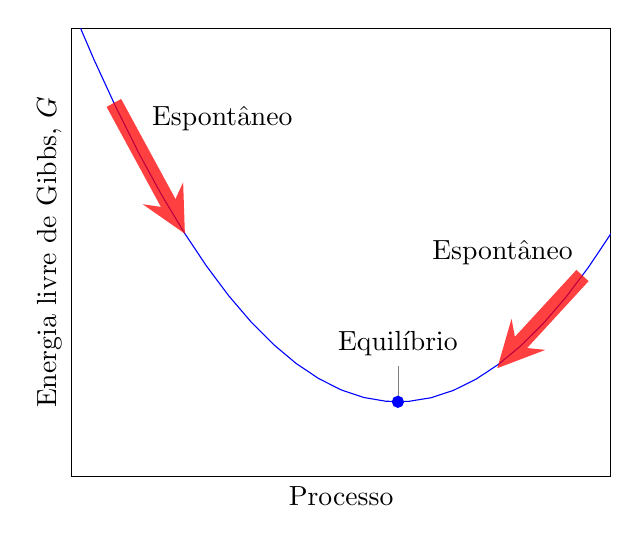
\begin{tikzpicture}
    \begin{axis}
        [
            grid = major,
            xlabel = {Processo},
            ylabel = {Energia livre de Gibbs, $G$},
            ytick = \empty,  
            xtick = \empty,
            xmin = -0.3, xmax = 3.5,
            ymin = -1, ymax = 5,
            domain = -0.3:3.5,
        ]
    \addplot [blue]
        { (x-2)^2 };

    \addplot [ mark=*, color=blue, only marks ] coordinates
        { (2, 0) };

    \begin{scope}[transparency group, opacity=0.75]
        \draw[-stealth, red, line width=0.6em] 
            (0,4) -- (0.5,2.25);
        \draw[-stealth, red, line width=0.6em] 
            (3.3,1.69) -- (2.7,0.45);
    \end{scope}
    
    \node [anchor = south west] at (axis cs:0.2,3.5) 
        { Espontâneo };

    \node [anchor = south east] at (axis cs:3.3,1.7) 
        { Espontâneo };

    \node[coordinate, pin={[fill=white] above:{Equilíbrio}}] 
        at (axis cs:2,0)   {};

    \end{axis}
\end{tikzpicture}
\caption{Variação da energia livre de Gibbs de uma mistura de reação com a composição. A mistura de reação tem a tendência espontânea de mudar na
direção da menor energia livre de Gibbs. Observe que \(\Delta G\) é a inclinação da linha em cada composição e que \(\Delta G^\circ\) é a diferença
entre as energias livres padrão molares dos reagentes puros e dos produtos puros.}
\end{figure}

O valor de \(\Delta G\) em um determinado ponto da reação é a diferença entre a energia livre de Gibbs molar dos produtos e dos reagentes \emph{nas
pressões parciais ou concentrações que eles têm naquele ponto}, ponderadas pelos coeficientes estequiométricos interpretados como a quantidade em
mols: \[
    \Delta G_\mathrm{r} 
        = \sum_\text{produtos} n_\mathrm{r} G_\mathrm{m} 
        - \sum_\text{reagentes} n_\mathrm{r} G_\mathrm{m}
\tag{3}
\] As energias livres de Gibbs molares \(G_\mathrm{m}\) dos reagentes e produtos mudam durante o curso da reação porque, quando somente os reagentes
estão presentes, cada molécula é cercada por moléculas de reagentes, mas, quando os produtos se formam, o ambiente de cada molécula também é alterado.
Como todos os valores de \(G_\mathrm{m}\) mudam, \(\Delta G\) varia com o andamento da reação. Vimos no Tópico 2D que a energia livre de Gibbs molar
de um gás ideal, \(\ce{J}\), está relacionada à pressão parcial, \(P_{\ce{J}}\), por \[
    G_{\mathrm{m}, \ce{J}} 
        = G_{\mathrm{m}, \ce{J}}^\circ + RT \ln \left( \dfrac{ P_{\ce{J}} }{ P^\circ } \right)
\] Argumentos termodinâmicos (que não serão reproduzidos aqui) mostram que uma expressão semelhante se aplica a solutos e substâncias puras. Em cada
caso, podemos escrever a energia livre de Gibbs molar de uma substância \(\ce{J}\) como \[
    G_{\mathrm{m}, \ce{J}} = G_{\mathrm{m}, \ce{J}}^\circ + RT \ln a_{\ce{J}}
\tag{4}
\] O valor de \(\Delta G\) em qualquer ponto da reação pode ser expresso a partir da composição da mistura de reação naquele ponto.

\begin{derivation}

\subsubsection{Como isso é feito?}

Para encontrar a expressão de \(\Delta G_\mathrm{r}^\circ\) da reação \[
    \ce{a A + b B <=> c C + d D } 
\] Insira a Equação 4b para cada substância na Equação 3b: \[
\begin{aligned}
    \Delta G_\mathrm{r} =&  
        + \big\{
            \overbrace{ c G_{\mathrm{m}, \ce{C}} + d G_{\mathrm{m}, \ce{D}} }^{\text{produtos}} 
        \big\}
        - 
        \big\{
            \overbrace{ a G_{\mathrm{m}, \ce{A}} + b G_{\mathrm{m}, \ce{B}} }^{\text{reagentes}} 
        \big\} 
        \\
        =& 
        + \big\{
            c \left[ G_{\mathrm{m}, \ce{C}}^\circ + RT \ln a_{\ce{C}} \right]
            + d \left[ G_{\mathrm{m}, \ce{D}}^\circ + RT \ln a_{\ce{D}} \right] 
        \big\}
        \\
        & 
        + \big\{
            a \left[ G_{\mathrm{m}, \ce{A}}^\circ + RT \ln a_{\ce{A}} \right]
            - b \left[ G_{\mathrm{m}, \ce{B}}^\circ + RT \ln a_{\ce{B}} \right]
        \big\}
\end{aligned}
\]

A combinação dos termos de energia livre leva à energia livre de Gibbs padrão da reação, \(\Delta G_\mathrm{r}^\circ\): \[
\begin{aligned}
        \Delta G_\mathrm{r} =&  
        \; \big\{
            \overbrace{ 
                c G_{\mathrm{m}, \ce{C}}^\circ 
                + d G_{\mathrm{m}, \ce{D}}^\circ
                - a G_{\mathrm{m}, \ce{A}}^\circ 
                - b G_{\mathrm{m}, \ce{B}}^\circ 
            }^{ \Delta G_\mathrm{r}^\circ }
        \big\}
        \\
        &
        + RT \big\{ 
            ( c \ln a_{\ce{C}} + d \ln a_{\ce{D}} ) 
            - ( a \ln a_{\ce{A}} + b \ln a_{\ce{B}} )
        \big\}
\end{aligned}
\] Logo, arrumando os quatro termos logarítmicos: \[
    \Delta G_\mathrm{r} = 
        \Delta G_\mathrm{r}^\circ 
        + RT \ln \dfrac{ (a_{\ce{C}})^c (a_{\ce{D}})^d }{ (a_{\ce{A}})^a (a_{\ce{B}})^b }  
\]

\end{derivation}

A expressão demonstrada acima pode ser escrita como \[
    \Delta G_\mathrm{r} = \Delta G_\mathrm{r}^\circ + RT \ln Q
\tag{5}
\] com o \textbf{quociente de reação}, \(Q\), definido como \[
    Q = \dfrac{ (a_{\ce{C}})^c (a_{\ce{D}})^d }{ (a_{\ce{A}})^a (a_{\ce{B}})^b }
\tag{6}
\] As Equações 5 e 6 mostram que a energia livre de Gibbs da reação varia com as atividades (pressões parciais de gases ou molaridades de solutos) dos
reagentes e produtos. A expressão de \(Q\) tem a mesma forma da expressão de \(K\), mas as atividades referem-se a \emph{qualquer} estágio da reação.

\begin{example}

\subsubsection{Cálculo da variação na energia livre de Gibbs a partir do quociente de reação}

Em \(\qty{25}{\unit{\degree C}}\), a reação \[
    \ce{ 2 SO2(g) + O2(g) <=> 2 SO3(g) }
\] tem energia livre de Gibbs padrão \(\Delta G_\mathrm{r}^\circ = \qty{-142}{\unit{kJ.mol^{-1}}}\). Em um experimento, a pressão parcial de cada gás
é \(\qty{100}{\unit{bar}}\).

\begin{enumerate}
\def\labelenumi{\alph{enumi}.}
\tightlist
\item
  \textbf{Calcule} a energia livre de Gibbs de reação.
\item
  \textbf{Avalie} a direção espontânea da reação nessas condições.
\end{enumerate}

\paragraph{Calcule o quociente de reação.}

De \(Q = (P_{\ce{SO3}})^2/(P_{\ce{SO2}})^2 P_{\ce{O2}}\) \[
    Q = \dfrac{ (\num{100})^2 }{ (\num{100})^2 \times (\num{100}) }
      = \num{0,01}
\]

\paragraph{Calcule a energia livre de reação.}

De \(\Delta G_\mathrm{r} = \Delta G_\mathrm{r}^\circ + RT \ln Q\) \[
\begin{aligned}
    \Delta G_\mathrm{r} &= 
        \Big\{ \num{-142} + (\num{8,3e-3}) \times (\num{298}) \times \ln \num{0,01} \Big\} \, \tfrac{\unit{kJ}}{\unit{mol}} \\
    &= \boxed{ \qty{-153}{\unit{kJ.mol^{-1}}} }
\end{aligned}
\] Como a energia livre de Gibbs de reação é negativa, a formação dos produtos é espontânea.

\end{example}

Você chegou agora ao ponto mais importante deste tópico. No equilíbrio, as atividades (pressões parciais ou molaridades) de todas as substâncias que
participam da reação estão em seu valor de equilíbrio. Neste ponto, a expressão de \(Q\) (em que as atividades estão em seu valor de equilíbrio)
torna-se igual à constante de equilíbrio, \(K\), da reação. No equilíbrio, \(Q = K\). A termodinâmica explicou a estranha forma de \(K\): ela é uma
consequência direta da Equação 5, que mostra como a energia livre de Gibbs de uma substância depende de sua composição e que \(K\) é simplesmente o
valor de \(Q\) quando todas as espécies estão em seus valores de equilíbrio.

Podemos dar, agora, mais um passo importante. Você sabe que, no equilíbrio, \(\Delta G_\mathrm{r} = 0\), e acabou de ver que, no equilíbrio,
\(Q = K\). Segue, da Equação 5, que, no equilíbrio, \[
    0 = \Delta G_\mathrm{r}^\circ + RT \ln K
\] e, portanto, que \[
    \Delta G_\mathrm{r}^\circ = -RT \ln K
\tag{7}
\] Essa equação fundamentalmente importante liga as quantidades termodinâmicas --- que estão disponíveis em tabelas de dados termodinâmicos --- e a
composição de um sistema em equilíbrio. Observe que:

\begin{itemize}
\tightlist
\item
  Se \(\Delta G_\mathrm{r}^\circ\) é negativo, \(\ln K\) deve ser positivo e, portanto, \(K > 1\); os produtos são favorecidos no equilíbrio.
\item
  Se \(\Delta G_\mathrm{r}^\circ\) é positivo, \(\ln K\) deve ser negativo e, portanto, \(K < 1\); os reagentes são favorecidos no equilíbrio.
\end{itemize}

\begin{think}

\subsubsection{Ponto para pensar}

Um catalisador dá um percurso de energia reduzida entre reagentes e produtos. A adição de um catalisador a uma reação altera a constante de
equilíbrio?

\end{think}

\begin{example}

\subsubsection{\texorpdfstring{Cálculo de \(K\) a partir da energia livre de Gibbs padrão de
reação}{Cálculo de K a partir da energia livre de Gibbs padrão de reação}}

Em \(\qty{25}{\unit{\degree C}}\), a reação \[
    \ce{ 1/2 H2(g) + 1/2 I2(g) <=> HI(g) }
\] tem energia livre de Gibbs padrão \(\Delta G_\mathrm{r}^\circ = \qty{+1,7}{\unit{kJ.mol^{-1}}}\).

\textbf{Calcule} a constante de equilíbrio da reação.

\paragraph{Calcule a constante de equilíbrio.}

De \(\ln K = - \Delta G_\mathrm{r}^\circ / RT\) \[
    \ln K = \dfrac{ \qty{1,7e3}{\tfrac{\unit{J}}{\unit{mol}}} }{ (\qty{8,3}{\tfrac{\unit{J}}{\unit{K.mol}}}) \times (\qty{298}{\unit{K}})  } = \num{-0,7}
\] Logo, \[
    K = e^{\num{-0,7}} = \boxed{ \num{0,5} }
\] Como esperado, a constante de equilíbrio é inferior a \(1\).

\end{example}

Agora você tem os elementos necessários para perceber por que algumas reações têm constantes de equilíbrio muito altas e, outras, muito baixas.
Segue-se de \[
    \Delta G_\mathrm{r}^\circ = \Delta H_\mathrm{r}^\circ - T \Delta S_\mathrm{r}^\circ
\] e \(\Delta G_\mathrm{r}^\circ = -RT \ln K\) que \[
    K = e^{-\Delta H_\mathrm{r}^\circ/RT} e^{\Delta S_\mathrm{r}^\circ/R}
\] Você pode ver agora que \(K\) pode ser pequeno se \(\Delta H_\mathrm{r}^\circ\) é positivo (porque \(e^{-x}\) é pequeno se \(x\) é positivo). Uma
reação endotérmica provavelmente terá \(K < 1\) e não formará uma grande quantidade de produto. Somente se \(\Delta S_\mathrm{r}^\circ\) for grande e
positivo, de forma que o fator seja grande, podemos esperar \(K > 1\) para uma reação endotérmica. Inversamente, se uma reação é fortemente
exotérmica, \(\Delta H_\mathrm{r}^\circ\) é grande e negativo. Portanto, você pode esperar que \(K > 1\) e que os produtos sejam favorecidos. Em
outras palavras, você pode esperar que as reações fortemente exotérmicas se completem.

\begin{quote}
O quociente de reação, \(Q\), tem a mesma forma de \(K\), a constante de equilíbrio, exceto que \(Q\) usa as atividades obtidas em um ponto arbitrário
da reação. A constante de equilíbrio está relacionada com a energia livre de Gibbs padrão de reação por \(\Delta G_\mathrm{r}^\circ = -RT \ln K\).
\end{quote}

\section{As formas alternativas da constante de equilíbrio}

O equilíbrio dinâmico atingido na síntese da amônia pode ser expresso de diversas maneiras: \[
    \ce{ N2(g) + 3 H2(g) <=> 2 NH3(g) }
\] ou \[
    \ce{ 4 NH3(g) <=> 2 N2(g) + 6 H2(g) }
\] Cada versão gera um valor diferente de \(K\). Talvez exista uma boa razão para escolher uma versão e não a outra e, então, é necessário converter
um valor tabulado para uma versão em um valor para a versão necessária. Outra questão emerge quando são usadas concentrações molares dos gases, porque
o procedimento termodinâmico para expressar uma constante de equilíbrio especifica que \(K\) é escrita em termos da pressão parcial de qualquer gás
que ocorra na reação, mas considerações de caráter prático muitas vezes significam que a concentração molar do gás é necessária. Como, então, a
constante de equilíbrio é expressa e relacionada com a versão termodinâmica?

\subsection{Os múltiplos da equação química}

As potências a que são elevadas as atividades na expressão das constantes de equilíbrio devem ser iguais aos coeficientes estequiométricos da equação
química, normalmente escritos com os menores coeficientes estequiométricos inteiros. Portanto, se os coeficientes estequiométricos de uma equação
química forem multiplicados por um fator, então a constante de equilíbrio deve refletir essa mudança. Por exemplo, em \(\qty{500}{\unit{K}}\), \[
    \ce{ H2(g) + I2(g) <=> 2 HI(g) } 
        \quad K_1 = \dfrac{ (P_{\ce{HI}})^2 }{ P_{\ce{H2}} P_{\ce{I2}} } = 160
\] Se a equação química for multiplicada por 2, a constante de equilíbrio torna-se \[
    \ce{ 2 H2(g) + 2 I2(g) <=> 4 HI(g) } \quad K_2
\] A constante de equilíbrio é escrita como \[
    K_2 = \dfrac{ (P_{\ce{HI}})^4 }{ (P_{\ce{H2}})^2 (P_{\ce{I2}})^2 } 
        = K_1^2 
        = 160^2
\] De modo geral, se uma equação química é multiplicada por um fator \(N\), \(K\) é elevado à \(N\)-ésima potência.

Agora, suponha que a equação original da reação seja invertida: \[
    \ce{ 2 HI(g) <=> H2(g) + I2(g) } \quad K_3
\] Essa equação ainda descreve o mesmo equilíbrio, mas escrevemos sua constante de equilíbrio como \[
    K_3 = \dfrac{ P_{\ce{H2}} P_{\ce{I2}} }{ (P_{\ce{HI}})^2 } 
        = \dfrac{1}{K_1} 
        = \dfrac{1}{160}
\]

\begin{info}

\subsubsection{Nota de boa prática}

Como esses exemplos mostram, é importante especificar a equação química a que a constante de equilíbrio se refere.

\end{info}

\subsection{As equações compostas}

Em alguns casos, uma equação química pode ser expressa como a soma de duas ou mais equações químicas. Por exemplo, considere as três reações em fase
gás: \[
\begin{aligned}
    \ce{ 2 P(g) + 3 Cl2(g) &<=> 2 PCl3(g) } 
        && K_1 = \dfrac{ (P_{\ce{PCl3}})^2 }{ (P_{\ce{P}})^2 (P_{\ce{Cl2}})^3 } \\
    \ce{ PCl3(g) + Cl2(g) &<=> PCl5(g) } 
        && K_2 = \dfrac{ P_{\ce{PCl3}} }{ P_{\ce{PCl3}} P_{\ce{Cl2}} } \\
    \ce{ 2 P(g) + 5 Cl2(g) &<=> 2 PCl5(g) } 
        && K_3 = \dfrac{ (P_{\ce{PCl3}})^2 }{ (P_{\ce{P}})^2 (P_{\ce{Cl2}})^5 }
\end{aligned}
\] A terceira reação é a soma das duas primeiras reações (a segunda foi multiplicada pelo fator 2): \[
\begin{aligned}
    \ce{ 2 P(g) + 3 Cl2(g) &<=> 2 PCl3(g) } \\
    \ce{ 2 PCl3(g) + 2 Cl2(g) &<=> 2 PCl5(g) } \\[1ex] 
    \hline \\[-2ex]
    \ce{ 2 P(g) + 5 Cl2(g) &<=> 2 PCl5(g) }
\end{aligned}
\] e a constante de equilíbrio, \(K_3\), da reação global pode ser escrita como o produto das constantes de equilíbrio das duas reações que, somadas,
dão a reação global. \[
    K_3 = \dfrac{ (P_{\ce{PCl3}})^2 }{ (P_{\ce{P}})^2 (P_{\ce{Cl2}})^5 }
        = \overbrace{ \dfrac{ (P_{\ce{PCl3}})^2 }{ (P_{\ce{P}})^2 (P_{\ce{Cl2}})^3 } }^{ K_1 } 
          \times
          \overbrace{ \dfrac{ (P_{\ce{PCl3}})^2 }{ (P_{\ce{P}})^2 (P_{\ce{Cl2}})^2 } }^{ K_2^2 }
        = K_1 K_2^2
\]

\begin{quote}
A constante de equilíbrio da reação total é o produto da constante de equilíbrio das reações parciais.
\end{quote}

\subsection{As concentrações molares dos gases}

A constante de equilíbrio é definida em termos das atividades, e estas são interpretadas em termos das pressões parciais dos gases ou das
concentrações molares dos solutos. \[
    \ce{a A + b B <=> c C + d D } 
        \quad K = \dfrac{ (a_{\ce{C}})^c (a_{\ce{D}})^d }{ (a_{\ce{A}})^a (a_{\ce{B}})^b }
\] Os gases sempre aparecem em \(K\) como os valores numéricos de suas pressões parciais em bar, e os solutos em uma fase condensada sempre aparecem
como os valores numéricos de suas concentrações molares em litros.

\begin{info}

\subsubsection{Nota de boa prática}

Em alguns casos, você encontrará uma constante de equilíbrio escrita como \(K_P\) para lembrá-lo de que ela está expressa em termos de pressões
parciais. O subscrito \(P\), entretanto, é desnecessário porque, por definição, as constantes de equilíbrio de reações em fase gás são expressas em
termos de pressões parciais.

\end{info}

No entanto, muitas vezes os equilíbrios gás-fase precisam ser discutidos em termos de concentrações molares, não pressões parciais, especialmente em
áreas da química como a cinética e a química atmosférica. Portanto, a constante de equilíbrio \(K_c\) é expressa como \[
     K_c = \ce{\frac{ [C]^c [D]^d }{ [A]^a [B]^b } }
\tag{9}
\] com cada concentração molar elevada a uma potência igual ao coeficiente estequiométrico da espécie correspondente na equação química. Por exemplo
para o equilíbrio na síntese da amônia, \[
    \ce{ N2(g) + 3 H2(g) <=> 2 NH3(g) } \quad K_c = \ce{ \frac{ [NH3]^2 }{ [N2] [H2]^3 } }
\]

\begin{warning}

\subsubsection{Atenção}

Você pode escolher \(K\) ou \(K_c\) para expressar a constante de equilíbrio de uma reação. Contudo, é importante lembrar que os cálculos de uma
constante de equilíbrio a partir de dados termodinâmicos (como as energias livres de formação de Gibbs, por exemplo) dão \(K\), não \(K_c\).

\end{warning}

Em alguns casos, você precisa conhecer \(K_c\) após ter calculado \(K\) a partir de dados termodinâmicos e, por isso, precisa também saber converter
as duas constantes uma na outra.

\begin{derivation}

\subsubsection{Como isso é feito?}

A estratégia geral usada para encontrar a relação entre \(K\) e \(K_c\) é substituir as pressões parciais que aparecem em \(K\) pelas concentrações
molares e, desse modo, obter \(K_c\). Para este cálculo, as atividades são escritas como \(P_{\ce{J}}/P^\circ\) e \(\ce{[J]}/c^\circ\) para acompanhar
as unidades, mantendo \(P^\circ = \qty{1}{\unit{bar}}\) e \(c^\circ = \qty{1}{\unit{mol.L^{-1}}}\).

O ponto de partida é supor que os gases sejam ideais e então escrever a forma completa da Equação 1: \[
    K = \dfrac{ (P_{\ce{A}}/P^\circ)^a (P_{\ce{B}}/P^\circ)^b }{ (P_{\ce{C}}/P^\circ)^c (P_{\ce{D}}/P^\circ)^d }
\] A concentração molar de cada gás é \(\ce{[J]} = n_{\ce{J}}/V\). Para um gás ideal, a lei dos gases ideais, \(P_{\ce{J}}V = n_{\ce{J}}RT\), pode ser
rearranjada para mostrar as concentrações de forma explícita: \[
    P_{\ce{J}} 
        = \dfrac{ n_{\ce{J}}RT }{ V } 
        = RT \times \left( \dfrac{ n_{\ce{J}} }{ V } \right ) 
        = RT \ce{[J]}
\] Quando essa expressão é substituída para cada gás na expressão de \(K\), ela se torna \[
    K = \ce{\frac{ [C]^c [D]^d }{ [A]^a [B]^b } }
        \left( \dfrac{RT}{P^\circ} \right)^{ (c + d) - (a + b) } 
\] Neste ponto, observe que \(K_c\), Equação 2, na forma completa pode ser escrita como (com \(c^\circ\) mostrado): \[
    K_c = \frac{ (\ce{[C]}/c^\circ)^c (\ce{[D]}/c^\circ)^d }{ (\ce{[A]}/c^\circ)^a (\ce{[B]}/c^\circ)^b }
\] Quando essa expressão é inserida na expressão de \(K\), o resultado é \[
    K = K_c \left( \dfrac{ c^\circ RT }{ P^\circ } \right)^{ (c + d) - (a + b) }
\]

\end{derivation}

Uma boa maneira de lembrar a forma geral da expressão que acabamos de derivar e outras semelhantes é escrevê-la como \[
    K = K_c \left( \dfrac{ c^\circ RT }{ P^\circ } \right)^{ \Delta n_\text{r, gás} }
\tag{10a}
\] em que \(\Delta n_\text{r, gás}\) é a variação (adimensional) dos coeficientes estequiométricos para as espécies na fase gás na reação química. Se
nenhum gás participa da reação ou os números de moléculas de gás são idênticos nos dois lados da equação química, então \(\Delta n_\text{r, gás} = 0\)
e \(K = K_c\). A mesma relação acontece entre \(Q\) e \(Q_c\), o quociente da reação em termos de concentrações. A Equação 4 normalmente é expressa de
forma mais simples como \[
    K = K_c \left( RT \right)^{\Delta n_\text{r, gás}}
\tag{10b}
\] mas a versão completa deixa claras as unidades e deveria ser usada nos cálculos.

\begin{example}

\subsubsection{\texorpdfstring{Conversão entre \(K\) e \(K_c\)}{Conversão entre K e K\_c}}

Em \(\qty{400}{\unit{\degree C}}\), a reação \[
    \ce{ 2 SO2(g) + O2(g) <=> 2 SO3(g) }
\] tem constante de equilíbrio \(\num{3e4}\).

\textbf{Calcule} o valor de \(K_c\) para essa reação a \(\qty{400}{\unit{\degree C}}\).

\paragraph{Calcule a variação dos coeficientes estequiométricos para as espécies na fase gás na reação.}

\[
    \Delta n_\text{r, gás} = 2 - (2 + 1) = -1
\]

\paragraph{\texorpdfstring{Calcule a constante de equilíbrio \(K_c\).}{Calcule a constante de equilíbrio K\_c.}}

De \(K = K_c \left( RT \right)^{\Delta n_\text{r, gás}}\) \[
\begin{aligned}
    K_c &= (\num{3e4}) 
            \times \left( \num{0,082} \times \num{673} \right)^{-(-1)} \\
        &= \boxed{ \num{1,7e6} }
\end{aligned}
\]

\end{example}

\begin{quote}
No caso de cálculos termodinâmicos, os equilíbrios em fase gás são expressos em termos de \(K\). No caso de cálculos práticos, porém, eles podem ser
expressos em termos de concentrações molares usando‑se a Equação 10.
\end{quote}

\section{Os cálculos de equilíbrio}

A constante de equilíbrio sumaria a composição de uma mistura de reação que atingiu o equilíbrio. Ela pode ser usada para predizer as pressões
parciais de cada espécie no equilíbrio ou avaliar as concentrações de reagentes e produtos, conhecendo-se as condições iniciais. Existem dois estágios
nesta discussão. O primeiro consiste em entender a importância qualitativa da magnitude da constante de equilíbrio. O segundo é o uso quantitativo da
constante para avaliar as concentrações ou as pressões parciais na mistura no equilíbrio.

\subsection{O progresso da reação}

Quando \(K\) é grande, a reação quase se completa antes de atingir o equilíbrio, e a mistura de reação no equilíbrio é formada quase que
exclusivamente pelos produtos. Quando \(K\) é pequena, o equilíbrio é atingido logo após o início da reação. Por exemplo, considere a reação \[
    \ce{ H2(g) + Cl2(g) <=> 2 HCl(g) } 
        \quad K = \dfrac{ (P_{\ce{HCl}})^2 }{ P_{\ce{H2}} P_{\ce{Cl2}} }
\] Experimentos mostraram que \(K = \num{4e18}\) em \(\qty{500}{\unit{K}}\). Tamanho valor de \(K\) indica que, quando o sistema atinge o equilíbrio,
a maior parte dos reagentes foi convertida em \(\ce{HCl}\). Na verdade, a reação praticamente se completa. Agora, imagine o equilíbrio \[
    \ce{ N2(g) + O2(g) <=> 2 NO(g) } 
        \quad K = \dfrac{ (P_{\ce{NO}})^2 }{ P_{\ce{N2}} P_{\ce{O2}} }
\] Experiências mostram que \(K = \num{3e-21}\) em \(\qty{800}{\unit{K}}\). O valor muito pequeno de \(K\) nos diz que o sistema atinge o equilíbrio
quando uma quantidade muito pequena do produto se formou. Os reagentes \(\ce{N2}\) e \(\ce{O2}\) permanecem como as espécies dominantes no sistema,
mesmo no equilíbrio.

Estes comentários sobre equações químicas escritas com os menores valores inteiros para os coeficientes estequiométricos podem ser resumidos da
seguinte maneira

\begin{itemize}
\tightlist
\item
  Valores grandes de \(K\) (maiores do que aproximadamente \(10^3\)): o equilíbrio favorece os produtos.
\item
  Valores intermediários de \(K\) (no intervalo aproximado de \(10^{-3}\) a \(10^3\)): o equilíbrio não favorece os reagentes nem os produtos.
\item
  Valores pequenos de \(K\) (inferiores a aproximadamente \(10^{-3}\)): o equilíbrio favorece os reagentes.
\end{itemize}

\begin{example}

\subsubsection{Cálculo da composição de equilíbrio}

Em uma mistura em equilíbrio em \(\qty{500}{\unit{K}}\) contendo \(\ce{HCl}\), \(\ce{Cl2}\) e \(\ce{H2}\), a pressão parcial de \(\ce{H2}\) é
\(\qty{4}{\unit{mPa}}\) e a de \(\ce{Cl2}\) é \(\qty{9}{\unit{mPa}}\). Nessa temperatura, a reação \[
    \ce{ H2(g) + Cl2(g) <=> 2 HCl(g) }
\] tem constante de equilíbrio \(K = \num{4e18}\).

\textbf{Calcule} a pressão parcial de \(\ce{HCl}\) no equilíbrio.

\paragraph{Calcule a pressão parcial do gás no equilíbrio.}

De \(K = (P_{\ce{HCl}})^2/P_{\ce{H2}}P_{\ce{Cl2}}\) \[
\begin{aligned}
    P_{\ce{HCl}} 
        &= \left( (\num{4e18}) \times (\num{4e-8}) \times (\num{9e-8}) \right)^{1/2} \\
        &= \boxed{ \qty{120}{\unit{bar}} }
\end{aligned}
\]

\end{example}

\begin{quote}
Se \(K\) é grande, os produtos são favorecidos no equilíbrio (o equilíbrio tende à direita); se \(K\) é pequeno, os reagentes são favorecidos (o
equilíbrio tende à esquerda).
\end{quote}

\subsection{A direção da reação}

Agora, suponha que o sistema estudado não esteja em equilíbrio. Por exemplo, você tem as concentrações de reagentes e produtos em algum estágio
arbitrário de uma reação, mas precisa saber se ela gerará mais produtos ou mais reagentes enquanto avança para o equilíbrio:

\begin{itemize}
\tightlist
\item
  Se \(Q < K\), as concentrações ou pressões parciais dos produtos estão muito baixas em relação às dos reagentes para a reação estar no equilíbrio.
  Assim, a reação tem a tendência de se processar na direção dos produtos.
\item
  Se \(Q = K\), a reação está na composição de equilíbrio e não tem tendência de mudar em nenhuma direção.
\item
  Se \(Q > K\), a reação inversa é espontânea, e os produtos tendem a se decompor nos reagentes.
\end{itemize}

\begin{warning}

\subsubsection{Atenção}

Observe que o critério de espontaneidade é \(\Delta G\), não \(\Delta G^\circ\). Se uma reação é espontânea ou não, depende do estágio que ela atinge.
Por essa razão, é melhor dizer que \(K > 1\) para uma reação com \(\Delta G_\mathrm{r}^\circ\) negativa, não que ela é espontânea. Entretanto, no caso
de reações com constantes de equilíbrio muito grandes, é pouco provável que a mistura de reagentes preparada no laboratório corresponda a \(Q > K\), e
é habitual referir-se a essas reações como \emph{espontâneas}.

\end{warning}

\begin{example}

\subsubsection{Predição da direção da reação}

Uma mistura de hidrogênio e iodo, ambos em \(\qty{55}{\unit{KPa}}\), e iodeto de hidrogênio, em \(\qty{78}{\unit{kPa}}\) foi introduzida em um
recipiente aquecido até \(\qty{783}{\unit{K}}\). Nessa temperatura, a reação \[
    \ce{ H2(g) + I2(g) <=> 2 HI(g) }
\] tem constante de equilíbrio \(K = \num{46}\).

\textbf{Avalie} se o \(\ce{HI}\) tem tendência a se formar ou a se decompor em \(\ce{H2}\) e \(\ce{I2}\).

\paragraph{Calcule o quociente de reação.}

De \(Q = (P_{\ce{HI}})^2/P_{\ce{H2}}P_{\ce{I2}}\) \[
    Q = \dfrac{ (\num{0,78})^2 }{ (\num{0,55}) \times (\num{0,55}) }
      = \num{2}
\] Como \(Q < K\), conclui-se que a reação tenderá a formar mais produtos e consumir os reagentes.

\end{example}

\begin{quote}
Uma reação apresenta tendência a formar produtos se \(Q < K\) e a formar reagentes se \(Q > K\).
\end{quote}

\subsection{Os cálculos com as constantes de equilíbrio}

A constante de equilíbrio de uma reação contém informações sobre a composição de equilíbrio em uma determinada temperatura. Entretanto, em muitos
casos, só a composição inicial da mistura de reação é conhecida, e você precisa predizer a composição em equilíbrio. Se você conhece o valor de \(K\),
é possível prever a composição no equilíbrio com base na estequiometria de reação. O procedimento mais fácil é elaborar uma tabela de equilíbrio, isto
é, uma tabela que mostra a composição inicial, as mudanças necessárias para atingir o equilíbrio em termos de uma quantidade desconhecida \(x\) e a
composição final do equilíbrio.

\begin{example}

\subsubsection{Cálculo da composição no equilíbrio com o uso de uma equação do segundo grau}

Em um reator de \(\qty{500}{\unit{mL}}\) foram colocados \(\qty{3,12}{\unit{g}}\) de \(\ce{PCl5}\). A amostra atingiu o equilíbrio com os produtos de
decomposição \(\ce{PCl3}\) e \(\ce{Cl2}\) em \(\qty{250}{\unit{\degree C}}\). A reação \[
    \ce{ PCl5(g) <=> PCl3(g) + Cl2(g) }
\] tem constante de equilíbrio \(K = \num{80}\) em \(\qty{250}{\unit{\degree C}}\).

\textbf{Calcule} a pressão parcial de \(\ce{PCl5}\) no equilíbrio.

\paragraph{\texorpdfstring{Calcule a quantidade inicial de \(\ce{PCl5}\).}{Calcule a quantidade inicial de \textbackslash ce\{PCl5\}.}}

De \(n = m/M\) \[
    n_{\ce{PCl5}, \text{início}} 
        = \dfrac{ \qty{3,12}{\unit{g}} }{ \qty{208}{\tfrac{\unit{g}}{\unit{mol}}} } 
        = \qty{0,015}{\unit{mol}}
\]

\paragraph{\texorpdfstring{Calcule a pressão parcial inicial de \(\ce{PCl5}\).}{Calcule a pressão parcial inicial de \textbackslash ce\{PCl5\}.}}

De \(PV = nRT\) \[
\begin{aligned}
    P_{\ce{PCl5}, \text{início}} 
        &= \dfrac{ (\qty{0,015}{\unit{mol}}) 
            \times (\qty{0,083}{\tfrac{\unit{bar.L}}{\unit{mol.K}}}) 
            \times (\qty{523}{\unit{K}}) }{ \qty{0,5}{\unit{L}} } \\
        &= \qty{1,3}{\unit{bar}}
\end{aligned}
\]

\paragraph{Escreva a expressão da constante de equilíbrio}

\[
    \ce{ PCl5(g) <=> PCl3(g) + Cl2(g) } 
        \quad K = \dfrac{ P_{\ce{PCl3}} P_{\ce{Cl2}} }{ P_{\ce{PCl5}} }
\]

\paragraph{Elabore uma tabela de equilíbrio.}

\begin{longtable}[]{@{}lccc@{}}
\toprule
& \(\ce{PCl5}\) & \(\ce{PCl3}\) & \(\ce{Cl2}\) \\
\midrule



início & \(\num{1,3}\) & \(0\) & \(0\) \\
reação & \(-x\) & \(+x\) & \(+x\) \\
equilíbrio & \(\num{1,3} - x\) & \(x\) & \(x\) \\
\end{longtable}

\paragraph{Insira os valores da tabela na expressão da constante de equilíbrio.}

\[
    K = 80 = \dfrac{ x^2 }{ \num{1,3} - x }
\] Resolvendo a equação do segundo grau para \(x\) obtemos \[
    x = \num{1,28} \text{ ou } x = \num{-81} 
\] Como as pressões parciais têm de ser positivas e como \(x\) é a pressão parcial de \(\ce{PCl3}\), selecione \(x = \num{1,28}\) como a solução.

\paragraph{\texorpdfstring{Calcule a pressão parcial de \(\ce{PCl5}\) no
equilíbrio.}{Calcule a pressão parcial de \textbackslash ce\{PCl5\} no equilíbrio.}}

De \(P_{\ce{PCl5}} = \qty{1,3}{\unit{bar}} - x\) \[
    P_{\ce{PCl5}} = \boxed{ \qty{0,02}{\unit{bar}} }
\]

\end{example}

Uma técnica de aproximação pode simplificar muito os cálculos quando a mudança de composição, \(x\), for menor do que cerca de \(5\%\) do valor
inicial. Para usá-la, suponha que \(x\) é desprezível quando adicionado ou subtraído de um número. Assim, todas as expressões da forma \(A + x\) ou
\(A - 2x\), por exemplo, podem ser substituídas por \(A\). Quando \(x\) aparece sozinho (quando não é adicionado ou subtraído de outro número), ele
não se altera. Logo, uma expressão como \((\num{0,1} - 2x)^2 x\) simplifica-se para \((\num{0,1})^2 x\), desde que \(2x \ll \num{0,1}\)
(especificamente, se \(2x < \num{0,005}\)). É importante verificar, no final dos cálculos, se o valor calculado de \(x\) é realmente inferior a cerca
de \(5\%\) dos valores iniciais. Se isso não ocorrer, então a equação deve ser resolvida sem a aproximação.

\begin{info}

\subsubsection{Nota de boa prática}

Um bom hábito é verificar a resposta, por meio da substituição da composição de equilíbrio na expressão de \(K\).

\end{info}

\begin{example}

\subsubsection{Cálculo da composição de equilíbrio por aproximação}

Uma mistura de \(\qty{0,5}{\unit{mol}}\) de \(\ce{N2}\) e \(\qty{1}{\unit{mol}}\) de \(\ce{O2}\) foi transferida para um balão de reação de volume
\(\qty{10}{\unit{L}}\) com formação de \(\ce{N2O}\) em \(\qty{800}{\unit{K}}\). A reação \[
    \ce{ 2 N2(g) + O2(g) <=> 2 N2O(g) }
\] tem constante de equilíbrio \(K = \num{3e-28}\) em \(\qty{800}{\unit{K}}\).

\textbf{Calcule} a pressão parcial de \(\ce{N2O}\) no equilíbrio.

\paragraph{Calcule as pressões parciais dos reagentes.}

De \(PV = nRT\) \[
\begin{aligned}
    P_{\ce{N2}} &= 
        \dfrac{ (\qty{0,5}{\unit{mol}}) \times (\qty{0,083}{\tfrac{\unit{bar.L}}{\unit{mol.K}}}) \times (\qty{800}{\unit{K}}) }{ \qty{10}{\unit{L}} } \\
    &= \qty{3,3}{\unit{bar}} \\
    P_{\ce{O2}} &= 
        \dfrac{ (\qty{1}{\unit{mol}}) \times (\qty{0,083}{\tfrac{\unit{bar.L}}{\unit{mol.K}}}) \times (\qty{800}{\unit{K}}) }{ \qty{10}{\unit{L}} } \\
    &= \qty{6,6}{\unit{bar}}
\end{aligned}
\]

\paragraph{Escreva a expressão da constante de equilíbrio.}

\[
    \ce{ 2 N2(g) + O2(g) <=> 2 N2O(g) }
        \quad K = \dfrac{ (P_{\ce{N2O}})^2 }{ (P_{\ce{N2}})^2 P_{\ce{O2}} }
\]

\paragraph{Elabore uma tabela de equilíbrio.}

\begin{longtable}[]{@{}lccc@{}}
\toprule
& \(\ce{N2}\) & \(\ce{O2}\) & \(\ce{N2O}\) \\
\midrule



início & \(\num{3,3}\) & \(\num{6,6}\) & \(0\) \\
reação & \(-2x\) & \(-x\) & \(+2x\) \\
equilíbrio & \(\num{3,3} - 2x\) & \(\num{6,6} - x\) & \(2x\) \\
\end{longtable}

\paragraph{Insira os valores da tabela na expressão da constante de equilíbrio.}

\[
    K = \dfrac{ (2x)^2 }{ (\num{3,3} - 2x)^2 (\num{6,6} - x) }
\]

\paragraph{\texorpdfstring{Hipótese. \(\num{3,3} - 2x \approx \num{3,3}\) e
\(\num{6,6} - x \approx \num{6,6}\).}{Hipótese. \textbackslash num\{3,3\} - 2x \textbackslash approx \textbackslash num\{3,3\} e \textbackslash num\{6,6\} - x \textbackslash approx \textbackslash num\{6,6\}.}}

Substituindo as hipóteses na expressão da constante de equilíbrio: \[
    K = \num{3e-28} = \dfrac{ (2x)^2 }{ (\num{3,3})^2 (\num{6,6}) }
\] Resolvendo a equação para \(x\) obtemos \[  
    x = \num{7,5e-14} 
\] O valor de \(2x\) é muito pequeno quando comparado com \(\num{3,3}\) (muito menor do que \(5\%\)), e nossa aproximação é válida.

\paragraph{\texorpdfstring{Calcule a pressão parcial de \(\ce{PCl5}\) no
equilíbrio.}{Calcule a pressão parcial de \textbackslash ce\{PCl5\} no equilíbrio.}}

De \(P_{\ce{N2O}} = 2x\) \[
    P_{\ce{N2O}} = \boxed{ \qty{1,5e-13}{\unit{bar}} }
\]

\end{example}

\begin{quote}
Para calcular a composição de uma reação em equilíbrio, organize uma tabela de equilíbrio em termos de mudanças nas pressões parciais ou nas
concentrações de reagentes e produtos, expresse a constante de equilíbrio conforme essas mudanças e resolva a equação resultante.
\end{quote}

\section{A resposta dos equilíbrios às mudanças das condições}

No início do século XX, a expectativa da eclosão da Primeira Guerra Mundial gerou uma desesperada busca por compostos de nitrogênio. Eventualmente, o
químico alemão Fritz Haber, em colaboração com o engenheiro químico de mesma nacionalidade Carl Bosch, encontrou uma forma econômica de utilizar o
nitrogênio do ar. Haber aqueceu nitrogênio e hidrogênio sob pressão na presença de ferro: \[
    \ce{ N2(g) + 3 H2(g) <=>[Fe] 2 NH3(g) }
\] O metal atua como um catalisador, uma substância que ajuda a reação a ocorrer mais rapidamente.

A reação avança até o equilíbrio, normalmente com uma concentração muito baixa de amônia. Haber buscava maneiras de aumentar a quantidade de produto
formada valendo-se do fato de que, como os equilíbrios químicos são dinâmicos, eles respondem a mudanças nas condições da reação.

\subsection{A adição e remoção de reagentes}

É possível predizer como a composição de uma reação em equilíbrio tende a mudar quando as condições se alteram usando o princípio identificado pelo
químico francês Henri Le Chatelier:

\begin{itemize}
\tightlist
\item
  \textbf{Princípio de Le Chatelier}: Quando uma perturbação é aplicada em um sistema em equilíbrio dinâmico, ele tende a se ajustar para reduzir ao
  mínimo o efeito da perturbação.
\end{itemize}

Esse princípio empírico (baseado em observações), no entanto, não é mais do que uma regra prática. Ele não dá uma explicação formal nem permite
predições \emph{quantitativas}. Entretanto, com o desenvolvimento do tópico, você entenderá as explicações cinéticas e termodinâmicas subjacentes e as
conclusões \emph{quantitativas} poderosas que podem ser deduzidas.

Imaginemos que a reação de síntese da amônia, reação A, atingiu o equilíbrio. Agora suponha que uma quantidade adicional de gás hidrogênio é bombeada
para o sistema. De acordo com o princípio de Le Chatelier, a reação tenderá a reduzir ao mínimo o efeito do aumento no número de moléculas de
hidrogênio através da reação do hidrogênio com o nitrogênio. Como resultado, forma-se mais amônia. Se, em vez de hidrogênio, tivéssemos adicionado
amônia, a reação tenderia a formar reagentes devido à amônia adicionada (Figura 3).

\begin{figure}
\centering

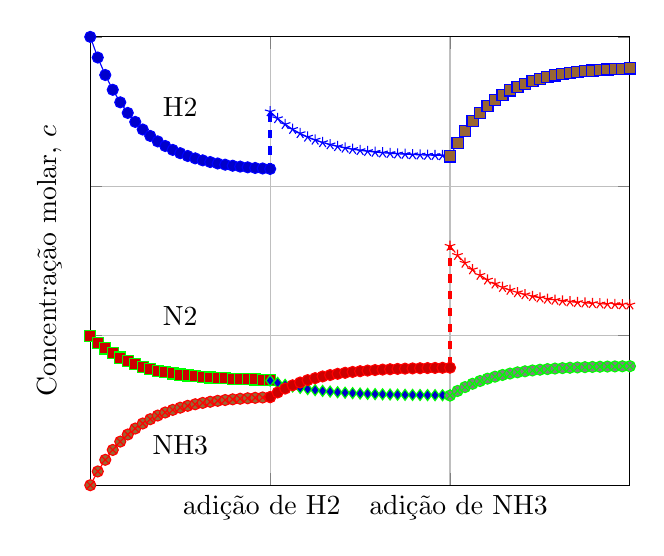
\begin{tikzpicture}
\begin{axis}
    [
        grid = major,
        ylabel = { Concentração molar, $c$ },
        xmin = 0, xmax = 12,
        ymin = 0, ymax = 3,
        xtick = {4, 8},
        xticklabels = { adição de \ce{H2} \;, \; adição de \ce{NH3} },
        yticklabels = \empty,
    ] 
    %%% PRIMEIRA PARTE
    \addplot+ [blue, domain = 0:4]
        { 
            3*exp(-x) + (1-exp(-x))*2.1
        };
    \addplot+ [green, domain = 0:4]
        { 
            1*exp(-x) + (1-exp(-x))*0.7
        };
    \addplot+ [red, domain = 0:4]
        { 
            2*(1-exp(-x)) - (1-exp(-x))*1.4
        };

    %%% SEGUNDA PARTE
    \draw [draw=blue, very thick, dashed]
        (axis cs: 4, 2.1) parabola 
        (axis cs: 4, 2.5);

    \addplot+ [blue, domain = 4:8]
        { 
            2.5*exp(4-x) + (1-exp(4-x))*2.2
        };
    \addplot+ [green, domain = 4:8]
        { 
            0.7*exp(4-x) + (1-exp(4-x))*0.6
        };
    \addplot+ [red, domain = 4:8]
        { 
            2*(1-exp(4-x)) - (1-exp(4-x))*1.8 + 0.59
        };

    %%% TERCEIRA PARTE
    \draw [draw=red, very thick, dashed]
        (axis cs: 8, 0.8) parabola 
        (axis cs: 8, 1.6);

    \addplot+ [blue, domain = 8:12]
        { 
            3*(1-exp(8-x)) - (1-exp(8-x))*2.4 + 2.2
        };
    \addplot+ [green, domain = 8:12]
        { 
            1*(1-exp(8-x)) - (1-exp(8-x))*0.8 + 0.6
        };
    \addplot+ [red, domain = 8:12]
        { 
            1.6*exp(8-x) + (1-exp(8-x))*1.2
        };

    \node [anchor = south] at (axis cs:2,2.4) 
        { \ce{H2} };
    \node [anchor = south] at (axis cs:2,1) 
        { \ce{N2} };
    \node [anchor = north] at (axis cs:2,0.4) 
        { \ce{NH3} };

\end{axis}
\end{tikzpicture}
    
\caption{Estes gráficos mostram as variações de composição que podem ser esperadas quando excesso de hidrogênio e, depois, amônia, são adicionados a
uma mistura de nitrogênio, hidrogênio e amônia em equilíbrio. Observe que a adição de hidrogênio resulta na formação de amônia, enquanto a adição de
amônia leva à decomposição de um pouco da amônia adicionada. Em ambos os casos, a mistura ajusta‑se a uma composição que está de acordo com a
constante de equilíbrio da reação.}
\end{figure}

\begin{think}

\subsubsection{Ponto para pensar}

Suponha que um dos produtos de uma reação que está em equilíbrio seja um sólido puro. Como o equilíbrio será afetado se um pouco do sólido for
removido? E se todo o sólido for removido?

\end{think}

A resposta de um sistema em equilíbrio após a adição ou remoção de uma substância pode ser explicada considerando-se as magnitudes relativas de \(Q\)
e \(K\). Quando são adicionados reagentes ou produtos, apenas \(Q\) varia, enquanto \(K\), uma característica da reação, mantém-se constante. No
equilíbrio, \(Q = K\) e, portanto, o valor de \(Q\) é afetado. Ele sempre tenderá a ser igual a \(K\) porque esta direção da mudança corresponde a uma
redução na energia livre de Gibbs.

\begin{itemize}
\tightlist
\item
  Quando reagentes são adicionados à mistura no equilíbrio, as concentrações dos reagentes no denominador de \(Q\) aumentam e, por isso, \(Q\) fica
  menor do que \(K\), temporariamente. Como \(Q < K\), a mistura de reação responde formando produtos e consumindo reagentes até \(Q = K\) outra vez.
  Isto é, quando reagentes são adicionados a um sistema em equilíbrio, ele reage convertendo reagentes em produtos.
\item
  Quando produtos são adicionados à mistura em equilíbrio, \(Q\) fica temporariamente maior do que \(K\), porque os produtos aparecem no numerador.
  Agora, como \(Q > K\), a mistura de reação responde formando reagentes à custa dos produtos, até \(Q = K\) outra vez. Isto é, quando produtos são
  adicionados ao sistema no equilíbrio, ele reage convertendo produtos em reagentes.
\end{itemize}

\begin{example}

\subsubsection{Predição do efeito da adição ou remoção de reagentes e produtos}

Considere a reação de produção de óxido nítrico \[
    \ce{ 4 NH3(g) + 5 O2(g) <=> 4 NO(g) + 6 H2O(g) }
\]

\textbf{Avalie} o efeito sobre a composição do equilíbrio das ações.

\begin{enumerate}
\def\labelenumi{\alph{enumi}.}
\tightlist
\item
  Remoção de \(\ce{NO}\).
\item
  Adição de \(\ce{NH3}\).
\item
  Adição de \(\ce{H2O}\).
\end{enumerate}

\paragraph{\texorpdfstring{Considere como cada alteração afetará o valor de \(Q\) e que mudança é necessária para restabelecer o
equilíbrio.}{Considere como cada alteração afetará o valor de Q e que mudança é necessária para restabelecer o equilíbrio.}}

\begin{enumerate}
\def\labelenumi{\alph{enumi}.}
\tightlist
\item
  A remoção de \(\ce{NO}\) (um produto) da mistura em equilíbrio reduz \(Q\) abaixo de \(K\), logo a reação se ajusta enquanto uma quantidade
  adicional de produtos é formada à custa dos reagentes.
\item
  Quando \(\ce{NH3}\) é adicionado ao sistema em equilíbrio, \(Q\) cai abaixo de \(K\), e, novamente, o equilíbrio se ajusta e produtos são formados à
  custa dos reagentes.
\item
  A adição de \(\ce{H2O}\) eleva \(Q\) acima de \(K\), com formação de reagentes à custa dos produtos.
\end{enumerate}

\end{example}

O princípio de Le Chatelier sugere um bom caminho para assegurar que a reação continue gerando uma dada substância: basta remover os produtos assim
que eles se formam. Na procura do equilíbrio, a reação avança na direção que gera mais produtos. Por essa razão, os processos industriais raramente
atingem o equilíbrio. Na síntese comercial da amônia, por exemplo, a amônia é removida continuamente fazendo-se circular a mistura em equilíbrio por
uma unidade de refrigeração na qual somente a amônia condensa. Portanto, o nitrogênio e o hidrogênio continuam a reagir para formar uma quantidade
adicional de produto.

\begin{example}

\subsubsection{Cálculo da composição no equilíbrio após a adição de um reagente}

Em um balão de \(\qty{500}{\unit{mL}}\), reação \[
    \ce{ PCl5(g) <=> PCl3(g) + Cl2(g) }
\] atingiu o equilíbrio em \(\qty{250}{\unit{\degree C}}\). As pressões parciais dos componentes no equilíbrio são
\(P_{\ce{PCl5}} = \qty{0,02}{\unit{bar}}\), \(P_{\ce{PCl3}} = \qty{1,28}{\unit{bar}}\) e \(P_{\ce{Cl2}} = \qty{1,28}{\unit{bar}}\). Foram adicionados
\(\qty{0,01}{\unit{mol}}\) de \(\ce{Cl2}\) à mistura no equilíbrio, então, o sistema entra em equilíbrio novamente.

\textbf{Calcule} a pressão parcial de \(\ce{PCl5}\) no equilíbrio.

\paragraph{Calcule o aumento de pressão parcial de cloro.}

De \(PV = nRT\) \[
\begin{aligned}
    \Delta P_{\ce{Cl2}} 
        &= \dfrac{ (\qty{0,01}{\unit{mol}}) \times (\qty{0,083}{\tfrac{\unit{bar.L}}{\unit{mol.L}}}) \times (\qty{523}{\unit{K}}) }{ \pu{(0,5 L)} }
        &= \qty{0,87}{\unit{bar}}
\end{aligned}
\] A pressão parcial total de cloro imediatamente após a adição do gás cloro é, portanto, \[
    P_{\ce{Cl2}, \text{início}} = \qty{1,28}{\unit{bar}} + \qty{0,870}{\unit{bar}} = \qty{2,15}{\unit{bar}}
\]

\paragraph{Escreva a expressão da constante de equilíbrio}

\[
    \ce{ PCl3(g) + Cl2(g) <=> PCl5(g) } 
        \quad K = \dfrac{ P_{\ce{PCl5}} }{ P_{\ce{PCl3}} P_{\ce{Cl2}} }
\]

\paragraph{Calcule a constante de equilíbrio}

De \(K = P_{\ce{PCl5}} / P_{\ce{PCl3}} P_{\ce{Cl2}}\) \[
    K = \dfrac{ (\num{0,02}) }{ (\num{1,28}) \times (\num{1,28}) } = \num{0,012}
\]

\paragraph{Elabore uma tabela de equilíbrio.}

\begin{longtable}[]{@{}lccc@{}}
\toprule
& \(\ce{PCl3}\) & \(\ce{Cl2}\) & \(\ce{PCl5}\) \\
\midrule



início & \(\num{1,28}\) & \(\num{2,15}\) & \(\num{0,02}\) \\
reação & \(-x\) & \(-x\) & \(+x\) \\
equilíbrio & \(\num{1,28} - x\) & \(\num{2,15} - x\) & \(\num{0,02} + x\) \\
\end{longtable}

\paragraph{Insira os valores da tabela na expressão da constante de equilíbrio.}

\[
    K = \num{0,012} 
      = \dfrac{ (\num{0,02} + x) }{ (\num{1,28} - x) \times (\num{2,15} - x) }
\] Resolvendo a equação do segundo grau para \(x\) obtemos \[
    x = \num{0,014} \text{ ou } x = \num{81} 
\] Como as pressões parciais têm de ser positivas, selecione \(x = \num{0,014}\) como a solução.

\paragraph{\texorpdfstring{Calcule a pressão parcial de \(\ce{PCl5}\) no
equilíbrio.}{Calcule a pressão parcial de \textbackslash ce\{PCl5\} no equilíbrio.}}

De \(P_{\ce{PCl5}} = \num{0,02} + x\) \[
    P_{\ce{PCl5}} = \boxed{ \qty{0,034}{\unit{bar}} }
\]

\end{example}

\begin{quote}
Quando a composição de equilíbrio é perturbada pela adição ou remoção de um reagente ou produto, a reação tende a ocorrer na direção que faz com que o
valor de \(Q\) torne‑se novamente igual a \(K\).
\end{quote}

\subsection{A compressão de uma mistura de reação}

Um equilíbrio em fase gás responde à compressão a redução de volume --- do recipiente da reação. De acordo com o princípio de Le Chatelier, a
composição tende a mudar para reduzir ao mínimo o efeito do aumento da pressão. Por exemplo, na dissociação de \(\ce{I2}\) para formar átomos de
\(\ce{I}\), \[
    \ce{ I2(g) <=> 2 I(g) }
\] \(\qty{1}{\unit{mol}}\) de moléculas do reagente na fase gás produz \(\qty{2}{\unit{mols}}\) de produto na fase gás. A reação direta aumenta o
número de partículas do recipiente e também a pressão total do sistema, e a reação inversa diminui a pressão. Logo, quando a mistura é comprimida, a
composição de equilíbrio tende a se deslocar na direção do reagente, \(\ce{I2}\), porque isso reduz ao mínimo o efeito do aumento da pressão. A
expansão provoca a resposta contrária, isto é, favorece a dissociação de \(\ce{I2}\) em átomos livres. Na formação da amônia, reação A,
\(\qty{2}{\unit{mols}}\) de moléculas de gás são produzidos a partir de \(\qty{4}{\unit{mols}}\) de moléculas de gás. Haber compreendeu que, para
aumentar o rendimento da amônia, seria preciso conduzir a síntese com gases fortemente comprimidos. O processo industrial utiliza pressões de
\(\qty{250}{\unit{atm}}\) ou mais.

O efeito da compressão sobre uma mistura em equilíbrio pode ser explicado mostrando que a compressão de um sistema altera os valores de pressão
parcial na expressão de \(K\), ainda que \(K\) não se altere.

\begin{derivation}

\subsubsection{Como isso é feito?}

Suponha que você queira descobrir o efeito da compressão sobre o equilíbrio \[
    \ce{ 2 NO2(g) <=> N2O4(g) }
\] Escreva a constante de equilíbrio na forma completa (para termos cuidado com as unidades) como: \[
    K = \dfrac{ (P_{\ce{N2O4}}/P^\circ) }{ (P_{\ce{NO2}}/P^\circ)^2 }
\] A seguir, como o foco deve ser o volume do sistema, considere que a compressão expressa \(K\) em termos do volume escrevendo
\(P_{\ce{J}} = n_{\ce{J}} RT/V\) para cada substância. \[
    K = \dfrac{ (n_{\ce{N2O4}}RT/VP^\circ) }{ (n_{\ce{NO2}}RT/VP^\circ)^2 } 
      = \dfrac{ n_{\ce{N2O4}} }{ (n_{\ce{NO2}})^2 } 
        \times 
        \dfrac{ P^\circ }{ RT }
        \times V
\] Como \(P^\circ/RT\) é constante, para que essa expressão permaneça constante quando o volume, \(V\), do sistema diminui, a razão
\(n_{\ce{N2O4}}/(n_{\ce{NO2}})^2\) deve aumentar. Isto é, a quantidade de \(\ce{NO2}\) deve diminuir e a quantidade de \(\ce{N2O4}\) deve aumentar.
Portanto, quando o volume do sistema diminui, o equilíbrio muda na direção do menor número total de moléculas na fase gás. Quando o sistema se
expande, uma quantidade adicional de \(\ce{NO2}\) seria produzida, e o equilíbrio se deslocaria na direção de um número total maior de moléculas do
gás.

\end{derivation}

\begin{example}

\subsubsection{Predição do efeito da compressão sobre o equilíbrio}

\textbf{Avalie} o efeito da compressão na composição do equilíbrio para as reações.

\begin{enumerate}
\def\labelenumi{\alph{enumi}.}
\tightlist
\item
  \(\ce{ 2 NO2(g) <=> N2O4(g) }\)
\item
  \(\ce{ N2(g) + O2(g) <=> 2 NO(g) }\)
\item
  \(\ce{ CH4(g) + H2O(g) <=> CO(g) + 3 H2(g) }\)
\item
  \(\ce{ CO2(g) + H2O(l) <=> H2CO3(aq) }\)
\end{enumerate}

\paragraph{Identifique o sentido em que há diminuição na quantidade de gás.}

\begin{enumerate}
\def\labelenumi{\alph{enumi}.}
\tightlist
\item
  Os produtos são favorecidos.
\item
  Não há efeito.
\item
  Os reagentes são favorecidos.
\item
  Os produtos são favorecidos.
\end{enumerate}

\end{example}

\begin{warning}

\subsubsection{Atenção}

Suponha que a pressão interna total no vaso de reação fosse aumentada bombeando argônio ou outro gás inerte, em volume constante. Como os gases que
reagem continuariam ocupando o mesmo volume, suas concentrações molares e suas pressões parciais permaneceriam inalteradas, apesar da presença de um
gás inerte. Nesse caso, portanto, ainda que os gases possam ser considerados ideais, a composição de equilíbrio não é afetada, embora a pressão total
tenha aumentado.

\end{warning}

\begin{quote}
A compressão de uma mistura de reação em equilíbrio tende a deslocar a reação na direção que reduz o número de moléculas em fase gás. O aumento da
pressão pela introdução de um gás inerte não afeta a composição em equilíbrio.
\end{quote}

\subsection{O equilíbrio e a temperatura}

A constante de equilíbrio de uma reação depende da temperatura. Duas observações experimentais resumem esta dependência. Sabe-se que, para reações
exotérmicas (que liberam calor), quando a temperatura é aumentada a composição da mistura em equilíbrio é deslocada em favor dos reagentes (\(K\)
diminui) e que o oposto ocorre em reações endotérmicas (que absorvem calor, \(K\) aumenta).

O princípio de Le Chatelier está de acordo com essas observações. Como a composição favorece os reagentes em uma reação exotérmica, a quantidade de
calor liberada é menor, o que pode ser visto como fator que contrabalança o aumento da temperatura. Da mesma forma, como a composição se desloca para
os produtos em uma reação endotérmica, a quantidade de calor absorvido é maior, o que ajuda a compensar o aumento da temperatura.

Um exemplo é a decomposição dos carbonatos. Uma reação como \[
    \ce{ CaCO3(s) -> CaO(s) + CO2(g) }
\] é fortemente endotérmica, e a pressão parcial de dióxido de carbono só é apreciável no equilíbrio se a temperatura for alta. Por exemplo, em
\(\qty{800}{\unit{\degree C}}\), a pressão parcial é \(\qty{0,22}{\unit{atm}}\) no equilíbrio. Se o aquecimento ocorre em um recipiente aberto, essa
pressão parcial nunca é atingida, porque o equilíbrio nunca é atingido. O gás se dispersa e o carbonato de cálcio decompõe-se completamente, deixando
um resíduo sólido de \(\ce{CaO}\). Entretanto, se o ambiente já for rico em dióxido de carbono, com a pressão parcial acima de
\(\qty{0,22}{\unit{atm}}\), então não ocorre decomposição: para cada molécula de \(\ce{CO2}\) que se forma, outra é reconvertida a carbonato. Esse
processo dinâmico é, provavelmente, o que acontece na superfície de Vênus, onde a pressão parcial do dióxido de carbono fica em torno de
\(\ce{87 atm}\). Essa alta pressão levou à especulação de que a superfície do planeta é rica em carbonatos, apesar da alta temperatura (em torno de
\(\qty{500}{\unit{\degree C}}\)).

\begin{example}

\subsubsection{Predição do efeito da temperatura sobre o equilíbrio}

\textbf{Avalie} como se comporta a composição de equilíbrio na síntese do trióxido de enxofre \[
    \ce{ 2 SO2(g) + O2(g) <=>[V2O5] 2 SO3(g) }
\] quando a temperatura aumenta.

\begin{longtable}[]{@{}lrr@{}}
\toprule
& \(\ce{SO2(g)}\) & \(\ce{SO3(g)}\) \\
\midrule



\(\Delta H_{\mathrm{f}}^\circ/\tfrac{\unit{kJ}}{\unit{mol}}\) & \(\num{-297}\) & \(\num{-396}\) \\
\end{longtable}

\paragraph{Calcule a entalpia padrão de reação.}

De \(\Delta H_\mathrm{r}^\circ = \sum_\text{produtos} n \Delta H^\circ_\mathrm{f} - \sum_\text{reagentes} n \Delta H^\circ_\mathrm{f}\) \[
   \Delta H_\mathrm{r}^\circ 
      = 2 \Delta H^\circ_{\mathrm{f}, \ce{SO3(g)}} 
        - 2 \Delta H^\circ_{\mathrm{f}, \ce{SO2(g)}}
\] logo, \[
\begin{aligned}
   \Delta H_\mathrm{r}^\circ
      &= \Big\{ 2 (\num{-396}) - 2 (\num{-297}) \Big\}\,\tfrac{\unit{kJ}}{\unit{mol}} \\
      &= \qty{-198}{\unit{kJ.mol^{-1}}}
\end{aligned}
\] Como a formação de \(\ce{SO3}\) é exotérmica, o aumento da temperatura da mistura no equilíbrio favorece a decomposição de \(\ce{SO3}\) em
\(\ce{SO2}\) e \(\ce{O2}\). Em consequência, as pressões do \(\ce{SO2}\) e do \(\ce{O2}\) vão aumentar e a do \(\ce{SO3}\) vai diminuir.

\end{example}

O efeito da temperatura na composição de equilíbrio é uma consequência da dependência da constante de equilíbrio com a temperatura.

\begin{derivation}

\subsubsection{Como isso é feito?}

As relações entre a constante de equilíbrio e a energia livre de Gibbs é \[
    \Delta G_\mathrm{r}^\circ = -RT \ln K
\] Introduzimos a definição de \(\Delta G_\mathrm{r}^\circ\) em termos de \(\Delta H_\mathrm{r}^\circ\) e \(\Delta S_\mathrm{r}^\circ\): \[
    \Delta G_\mathrm{r}^\circ = \Delta H_\mathrm{r}^\circ - T \Delta S_\mathrm{r}^\circ
\] para dar \[
    \ln K = \dfrac{ \Delta S_\mathrm{r}^\circ }{ R } 
          - \dfrac{ \Delta H_\mathrm{r}^\circ }{ R T } 
\] As constantes de equilíbrio \(K_1\) e \(K_2\) em duas temperaturas \(T_1\) e \(T_2\) são \[
\begin{aligned}
    \text{Em $T_1$:} \quad \ln K_1 
        &= \dfrac{ \Delta S_\mathrm{r}^\circ }{ R } 
         - \dfrac{ \Delta H_\mathrm{r}^\circ }{ R T_1 } \\
    \text{Em $T_2$:} \quad \ln K_2 
        &= \dfrac{ \Delta S_\mathrm{r}^\circ }{ R } 
         - \dfrac{ \Delta H_\mathrm{r}^\circ }{ R T_2 }
\end{aligned}
\] É razoável considerar \(\Delta H_\mathrm{r}^\circ\) e \(\Delta S_\mathrm{r}^\circ\) aproximadamente independentes da temperatura na faixa de
interesse. Quando essa aproximação é feita, podemos eliminar \(\Delta S_\mathrm{r}^\circ/R\) subtraindo a primeira equação da segunda: \[
    \overbrace{ \ln K_2 - \ln K_1 }^{ \ln (K_2/K_1) } 
        = -\dfrac{ \Delta H^\circ_\mathrm{r} }{ R } 
            \left( \dfrac{1}{T_2} - \dfrac{1}{T_1} \right)
\]

\end{derivation}

A expressão que acabamos de demonstrar é uma versão quantitativa do princípio de Le Chatelier para o efeito da temperatura. Normalmente ela é
rearranjada na equação de van't Hoff: \[
    \ln \left( \dfrac{K_2}{K_1} \right)
        = -\dfrac{ \Delta H^\circ_\mathrm{r} }{ R } 
            \left( \dfrac{1}{T_2} - \dfrac{1}{T_1} \right)
\tag{11}
\] Nesta expressão, \(K_1\) é a constante de equilíbrio quando a temperatura é \(T_1\), e \(K_2\) é a constante de equilíbrio quando a temperatura é
\(T_2\).

\begin{info}

\subsubsection{O que esta equação revela}

Se a reação é endotérmica, então \(\Delta H^\circ_\mathrm{r}\) é positivo. Se \(T_2 > T_1\), então \(1/T_2 < 1/T_1\) e o termo entre parênteses também
é positivo. Portanto, \(\ln(K_2/K_1)\) é positivo, ou seja, \(K_2/K_1\) \textgreater{} 1 e, portanto, \(K_2 > K_1\). Em outras palavras, o aumento de
temperatura favorece a formação de produtos se a reação for endotérmica. O efeito oposto ocorre para uma reação exotérmica, porque
\(\Delta H^\circ_\mathrm{r}\) é negativo. Portanto, a equação de van't Hoff explica o princípio de Le Chatelier para o efeito da temperatura no
equilíbrio.

\end{info}

\begin{example}

\subsubsection{Cálculo da constante de equilíbrio em diferentes temperaturas}

Em \(\qty{298}{\unit{K}}\), a reação \[
    \ce{ N2(g) + 3 H2(g) <=> 2 NH3(g) }
\] tem entalpia \(\qty{-90}{\unit{kJ.mol^{-1}}}\) e constante de equilíbrio \(\num{7e5}\).

\textbf{Calcule} o valor da constante de equilíbrio em \(\qty{400}{\unit{K}}\).

\paragraph{Use a equação de van't Hoff.}

De \(\ln \left( \frac{K_2}{K_1} \right) = -\frac{ \Delta H^\circ_\mathrm{r} }{ R } \left( \frac{1}{T_2} - \frac{1}{T_1} \right)\) \[
\begin{aligned}
    \ln \left( \dfrac{K_2}{K_1} \right) 
        &= -\dfrac{ (\qty{-90e3}{\tfrac{\unit{J}}{\unit{mol}}}) }{ \qty{8,3}{\tfrac{\unit{J}}{\unit{K.mol}}}  } \left( \dfrac{1}{ \qty{298}{\unit{K}} } - \dfrac{1}{ \qty{400}{\unit{K}} } \right) \\
        &= \num{-9,5}
\end{aligned}
\] logo, \[
    K_2 = (\num{7e5}) \times e^{-9,5} = \boxed{ 50 }
\]

\end{example}

\begin{warning}

\subsubsection{Atenção}

Quando se usa a equação de van't Hoff para reações na fase gás, a constante de equilíbrio deve ser \(K\), não \(K_c\). Se você precisa de um novo
valor de \(K_c\) para uma reação em fase gás, você precisa converter \(K_c\) em \(K\) na temperatura inicial. Depois, use a equação de van't Hoff para
calcular o valor de \(K\) na nova temperatura e, finalmente, converta \(K\) em \(K_c\) usando o novo valor de \(K_c\), na nova temperatura.

\end{warning}

\begin{quote}
O aumento da temperatura de uma reação exotérmica reduz o valor de \(K\). O aumento da temperatura de uma reação endotérmica eleva o valor de \(K\). A
equação de van't Hoff expressa esse efeito de forma quantitativa.
\end{quote}

\section*{Problemas}

\begin{problem}[
	id={2F01},
	path={/home/braun/Documents/Developer/braunchem/data/problems/Q2/2F/2F01}
]
Considere as proposições a respeito de uma reação reversível.

\begin{enumerate}
\def\labelenumi{\arabic{enumi}.}
\tightlist
\item
  Uma reação para quando atinge o equilíbrio.
\item
  Uma reação em equilíbrio não é afetada pelo aumento da concentração de produtos.
\item
  Se a reação começa com maior pressão dos reagentes, a constante de equilíbrio será maior.
\item
  Se a reação começa com concentrações maiores de reagentes, as concentrações de equilíbrio dos produtos serão maiores.
\end{enumerate}

\textbf{Assinale} a alternativa que relaciona as proposições \emph{corretas}.
\autochoices{\textbf{3}}{\textbf{4}}{\textbf{1} e \textbf{4}}{\textbf{2} e \textbf{4}}{\textbf{3} e \textbf{4}}
\end{problem}


\begin{problem}[
	id={2F02},
	path={/home/braun/Documents/Developer/braunchem/data/problems/Q2/2F/2F02}
]
Considere as proposições a respeito de uma reação reversível.

\begin{enumerate}
\def\labelenumi{\arabic{enumi}.}
\tightlist
\item
  Em uma reação de equilíbrio, a reação inversa só ocorre quando todos os reagentes tiverem sido convertidos em produtos.
\item
  As concentrações de equilíbrio serão as mesmas se começarmos uma reação com os reagentes puros ou com os produtos puros.
\item
  As velocidades das reações direta e inversa são iguais no equilíbrio.
\item
  Se a energia livre de Gibbs é maior do que a energia livre padrão de reação, a reação avança até o equilíbrio.
\end{enumerate}

\textbf{Assinale} a alternativa que relaciona as proposições \emph{corretas}.
\autochoices{\textbf{2}}{\textbf{3}}{\textbf{2} e \textbf{3}}{\textbf{1}, \textbf{2} e \textbf{3}}{\textbf{2}, \textbf{3} e \textbf{4}}
\end{problem}


\begin{problem}[
	id={2F03},
	path={/home/braun/Documents/Developer/braunchem/data/problems/Q2/2F/2F03}
]
Considere a reação: {\[
    \ce{ 4 NH3(g) + 5 O2(g) <=> 4 NO(g) + 6 H2O(g) }
\]} \textbf{Assinale} a alternativa com a constante de equilíbrio da reação.
\autochoices{{\(\dfrac{ P_{\ce{NO}} }{ P_{\ce{NH3}} P_{\ce{O2}} }\)}
}{{\(\dfrac{ P_{\ce{NO}} P_{\ce{H2O}} }{ P_{\ce{NH3}} P_{\ce{O2}} }\)}
}{{\(\dfrac{ (P_{\ce{NO}})^4 }{ (P_{\ce{NH3}})^4 (P_{\ce{O2}})^5 }\)}
}{{\(\dfrac{ (P_{\ce{NO}})^4 (P_{\ce{H2O}})^6 }{ (P_{\ce{NH3}})^4 (P_{\ce{O2}})^5 }\)}
}{{\(\dfrac{ (P_{\ce{NH3}})^4 (P_{\ce{O2}})^5 }{ (P_{\ce{NO}})^4 (P_{\ce{H2O}})^6 }\)}
}
\end{problem}


\begin{problem}[
	id={2F04},
	path={/home/braun/Documents/Developer/braunchem/data/problems/Q2/2F/2F04}
]
Considere a reação: {\[
    \ce{ 2 H2S(g) + 3 O2(g) <=> 2 SO2(g) + 2 H2O(g) }
\]} \textbf{Assinale} a alternativa com a constante de equilíbrio da reação.
\autochoices{{\(\dfrac{ P_{\ce{SO2}} }{ P_{\ce{H2S}} P_{\ce{O2}} }\)}
}{{\(\dfrac{ P_{\ce{SO2}} P_{\ce{H2O}} }{ P_{\ce{H2S}} P_{\ce{O2}} }\)}
}{{\(\dfrac{ (P_{\ce{SO2}})^2 }{ (P_{\ce{H2S}})^2 (P_{\ce{O2}})^3 }\)}
}{{\(\dfrac{ (P_{\ce{SO2}})^2 (P_{\ce{H2O}})^2 }{ (P_{\ce{H2S}})^2 (P_{\ce{O2}})^3 }\)}
}{{\(\dfrac{ (P_{\ce{H2S}})^2 (P_{\ce{O2}})^3 }{ (P_{\ce{SO2}})^2 (P_{\ce{H2O}})^2 }\)}
}
\end{problem}


\begin{problem}[
	id={2F05},
	path={/home/braun/Documents/Developer/braunchem/data/problems/Q2/2F/2F05}
]
Considere a reação: {\[
    \ce{ Ni(s) + 4 CO(g) <=> Ni(CO)4(g) }
\]} \textbf{Assinale} a alternativa com a constante de equilíbrio da reação.
\autochoices{{\(\dfrac{ P_{\ce{Ni(CO)4}} }{ P_{\ce{CO}} }\)}
}{{\(\dfrac{ P_{\ce{Ni(CO)4}} }{ (P_{\ce{CO}})^4 }\)}
}{{\(\dfrac{ P_{\ce{Ni(CO)4}} }{ P_{\ce{Ni}} (P_{\ce{CO}})^4 }\)}
}{{\(\dfrac{ P_{\ce{Ni(CO)4}} }{ d_{\ce{Ni}} (P_{\ce{CO}})^4 }\)}
}{{\(\dfrac{ P_{\ce{Ni(CO)4}} }{ \ce{[Ni]} (P_{\ce{CO}})^4 }\)}
}
\end{problem}


\begin{problem}[
	id={2F06},
	path={/home/braun/Documents/Developer/braunchem/data/problems/Q2/2F/2F06}
]
Considere a reação: {\[
    \ce{ P4(s) + 5 O2(g) <=> P4O10(s) }
\]} \textbf{Assinale} a alternativa com a constante de equilíbrio da reação.
\autochoices{{\(\dfrac{ 1 }{ P_{\ce{O2}} }\)}
}{{\(\dfrac{ 1 }{ (P_{\ce{O2}})^5 }\)}
}{{\(\dfrac{ P_{\ce{P4O10}} }{ P_{\ce{P4}} (P_{\ce{O2}})^5 }\)}
}{{\(\dfrac{ d_{\ce{P4O10}} }{ d_{\ce{P4}} (P_{\ce{O2}})^5 }\)}
}{{\(\dfrac{ \ce{[P4O10]} }{ \ce{[P4]} (P_{\ce{O2}})^5 }\)}
}
\end{problem}


\begin{problem}[
	id={2F07},
	path={/home/braun/Documents/Developer/braunchem/data/problems/Q2/2F/2F07}
]
Considere a reação: {\[
    \ce{ 2 AgNO3(aq) + 2 NaOH(aq) <=> 2 Ag2O(s) + 2 NaNO3(aq) +
H2O(l) }
\]} \textbf{Assinale} a alternativa com a constante de equilíbrio da reação.
\autochoices{{\(\dfrac{ 1 }{ \ce{[Ag^+]} \ce{[OH^-]} }\)}
}{{\(\dfrac{ 1 }{ \ce{[Ag^+]}^2 \ce{[OH^-]}^2 }\)}
}{{\(\dfrac{ \ce{[H2O]} }{ \ce{[Ag^+]}^2 \ce{[OH^-]}^2 }\)}
}{{\(\dfrac{ \ce{[Ag2O]}^2 \ce{[NaNO3]}^2 }{ \ce{[AgNO3]}^2 \ce{[NaOH]}^2 }\)}
}{{\(\dfrac{ \ce{[Ag2O]}^2 \ce{[NaNO3]}^2 \ce{[H2O]} }{ \ce{[AgNO3]}^2 \ce{[NaOH]}^2 }\)}
}
\end{problem}


\begin{problem}[
	id={2F08},
	path={/home/braun/Documents/Developer/braunchem/data/problems/Q2/2F/2F08}
]
Considere a reação: {\[
    \ce{ Zn(s) + 2 HCl(aq) <=> ZnCl2(aq) + H2(g) }
\]} \textbf{Assinale} a alternativa com a constante de equilíbrio da reação.
\autochoices{{\(\dfrac{ \ce{[ZnCl]} P_{\ce{H2}} }{ \ce{[HCl]}^2 }\)}
}{{\(\dfrac{ \ce{[Zn^{2+}]} \ce{[H2]} }{ \ce{[H^+]}^2 }\)}
}{{\(\dfrac{ \ce{[Zn^{2+}]} P_{\ce{H2}} }{ \ce{[H^+]}^2 }\)}
}{{\(\dfrac{ \ce{[ZnCl]} P_{\ce{H2}} }{ \ce{[Zn]} \ce{[HCl]}^2 }\)}
}{{\(\dfrac{ \ce{[Zn^{2+}]} P_{\ce{H2}} }{ \ce{[Zn]} \ce{[H^+]}^2 }\)}
}
\end{problem}


\begin{problem}[
	id={2F09},
	path={/home/braun/Documents/Developer/braunchem/data/problems/Q2/2F/2F09}
]
Coloca-se uma amostra de {\(\qty{0,1}{\unit{mol}}\)} de ozônio puro, {\(\ce{O3}\)}, em um recipiente fechado de {\(\qty{1}{\unit{L}}\)} de deixa-se
que a reação atinja o equilíbrio: {\[
    \ce{ 2 O3(g) <=> 3 O2(g) }
\]} Em seguida, uma amostra de {\(\qty{0,5}{\unit{mol}}\)} de {\(\unit{O^{3}}\)} puro é colocado em um segundo recipiente de {\(\qty{1}{\unit{L}}\)},
na mesma temperatura e deixa-se que atinja o equilíbrio.

Considere as quantidades:

\begin{enumerate}
\def\labelenumi{\arabic{enumi}.}
\tightlist
\item
  Quantidade de {\(\ce{O2}\)}.
\item
  Pressão parcial de {\(\ce{O2}\)}.
\item
  Razão {\(P_{\ce{O2}}/P_{\ce{O3}}\)}.
\item
  Razão {\((P_{\ce{O2}})^3/(P_{\ce{O3}})^2\)}.
\end{enumerate}

\textbf{Assinale} a alternativa que relaciona as quantidades que serão \emph{iguais} nos dois recipientes no equilíbrio.
\autochoices{\textbf{3}}{\textbf{4}}{\textbf{1} e \textbf{4}}{\textbf{2} e \textbf{4}}{\textbf{3} e \textbf{4}}
\end{problem}


\begin{problem}[
	id={2F10},
	path={/home/braun/Documents/Developer/braunchem/data/problems/Q2/2F/2F10}
]
Coloca-se uma amostra de {\(\qty{0,1}{\unit{mol}}\)} de {\(\ce{H2}\)} e {\(\qty{0,1}{\unit{mol}}\)} de {\(\ce{Br2}\)} em um recipiente fechado de
{\(\qty{2}{\unit{L}}\)} de deixa-se que a reação atinja o equilíbrio: {\[
    \ce{ H2(g) + Br2(g) <=> 2 HBr(g) }
\]} Em seguida, uma amostra de {\(\qty{0,2}{\unit{mol}}\)} de {\(\ce{H2}\)} e {\(\qty{0,1}{\unit{mol}}\)} de {\(\ce{Br2}\)} é colocado em um segundo
recipiente de {\(\qty{2}{\unit{L}}\)}, na mesma temperatura e deixa-se que atinja o equilíbrio.

Considere as quantidades:

\begin{enumerate}
\def\labelenumi{\arabic{enumi}.}
\tightlist
\item
  Quantidade de {\(\ce{Br2}\)}.
\item
  Pressão parcial de {\(\ce{H2}\)}.
\item
  Razão {\(P_{\ce{HBr}}/P_{\ce{Br2}}\)}.
\item
  Pressão total no recipiente.
\end{enumerate}

\textbf{Assinale} a alternativa que relaciona as quantidades que serão \emph{iguais} nos dois recipientes no equilíbrio.
\autochoices{\textbf{1}, \textbf{2} e \textbf{3}}{\textbf{1}, \textbf{2} e \textbf{4}}{\textbf{1}, \textbf{3} e \textbf{4}}{\textbf{2}, \textbf{3} e \textbf{4}}{\textbf{1}, \textbf{2}, \textbf{3} e \textbf{4}}
\end{problem}


\begin{problem}[
	id={2F11},
	path={/home/braun/Documents/Developer/braunchem/data/problems/Q2/2F/2F11}
]
Considere a reação: {\[
    \ce{ 2 NO(g) + O2(g) <=> 2 NO2(g) }
\]} \textbf{Assinale} a alternativa que mais se aproxima da constante de equilíbrio para a reação em {\(\qty{25}{\unit{\degree C}}\)}.
\autochoices{\(\num{1,8E-13}\)}{\(\num{6,5E-13}\)}{\(\num{2,3E-12}\)}{\(\num{8,1E-12}\)}{\(\num{2,9E-11}\)}\paragraph{Dados}\small 
\begin{datalist}
[start = 1](2)\item $\Delta G_\mathrm{f}^{\circ}(\ce{NO2,\,\text{g}}) = \qty{51.3}{\tfrac{\unit{kJ}}{\unit{mol}}}$
\item $\Delta G_\mathrm{f}^{\circ}(\ce{NO,\,\text{g}}) = \qty{86.6}{\tfrac{\unit{kJ}}{\unit{mol}}}$
\end{datalist}

\end{problem}


\begin{problem}[
	id={2F12},
	path={/home/braun/Documents/Developer/braunchem/data/problems/Q2/2F/2F12}
]
Considere a reação: {\[
    \ce{ N2O4(g) <=> 2 NO2(g) }
\]} \textbf{Assinale} a alternativa que mais se aproxima da constante de equilíbrio para a reação em {\(\qty{25}{\unit{\degree C}}\)}.
\autochoices{\(\num{0,081}\)}{\(\num{0,11}\)}{\(\num{0,15}\)}{\(\num{0,20}\)}{\(\num{0,28}\)}\paragraph{Dados}\small 
\begin{datalist}
[start = 1](2)\item $\Delta H_\mathrm{f}^{\circ}(\ce{NO2,\,\text{g}}) = \qty{33.2}{\tfrac{\unit{kJ}}{\unit{mol}}}$
\item $\Delta H_\mathrm{f}^{\circ}(\ce{N2O4,\,\text{g}}) = \qty{9.16}{\tfrac{\unit{kJ}}{\unit{mol}}}$
\item $S_\mathrm{m}^{\circ}(\ce{NO2,\,\text{g}}) = \qty{240}{\tfrac{\unit{J}}{\unit{K.mol}}}$
\item $S_\mathrm{m}^{\circ}(\ce{N2O4,\,\text{g}}) = \qty{304}{\tfrac{\unit{J}}{\unit{K.mol}}}$
\end{datalist}

\end{problem}


\begin{problem}[
	id={2F13},
	path={/home/braun/Documents/Developer/braunchem/data/problems/Q2/2F/2F13}
]
Considere a reação em {\(\qty{500}{\unit{K}}\)}: {\[
    \ce{ H2(g) + I2(g) <=> 2 HI(g) } \quad \Delta
G^\circ_\mathrm{r} = \qty{-21}{\tfrac{\unit{kJ}}{\unit{mol}}}
\]} Em um experimento as pressões parciais dos gases são {\(\pu{P_{\ce{H2}}} = \qty{1,5}{\unit{bar}}\)},
{\(\pu{P_{\ce{I2}}} = \qty{0,88}{\unit{bar}}\)} e {\(\pu{P_{\ce{HI}}} = \qty{0,065}{\unit{bar}}\)}.

\textbf{Assinale} a alternativa que mais se aproxima da energia livre de reação.
\autochoices{\(\qty{-8,2}{\unit{kJ.mol^{-1}}}\)}{\(\qty{-13}{\unit{kJ.mol^{-1}}}\)}{\(\qty{-19}{\unit{kJ.mol^{-1}}}\)}{\(\qty{-29}{\unit{kJ.mol^{-1}}}\)}{\(\qty{-45}{\unit{kJ.mol^{-1}}}\)}
\end{problem}


\begin{problem}[
	id={2F14},
	path={/home/braun/Documents/Developer/braunchem/data/problems/Q2/2F/2F14}
]
Considere a reação em {\(\qty{400}{\unit{K}}\)}: {\[
    \ce{ N2O4(g) <=> 2 NO2(g) } \quad K = \num{40}
\]} Em um experimento as pressões parciais dos gases são {\(\pu{P_{\ce{N2}}} = \qty{4,2}{\unit{bar}}\)},
{\(\pu{P_{\ce{H2}}} = \qty{1,8}{\unit{bar}}\)} e {\(\pu{P_{\ce{NH3}}} = \qty{20}{\unit{bar}}\)}.

\textbf{Assinale} a alternativa que mais se aproxima da energia livre de reação.
\autochoices{\(\qty{-2,7}{\unit{kJ.mol^{-1}}}\)}{\(\qty{-3,5}{\unit{kJ.mol^{-1}}}\)}{\(\qty{-4,5}{\unit{kJ.mol^{-1}}}\)}{\(\qty{-5,7}{\unit{kJ.mol^{-1}}}\)}{\(\qty{-7,4}{\unit{kJ.mol^{-1}}}\)}
\end{problem}


\begin{problem}[
	id={2F15},
	path={/home/braun/Documents/Developer/braunchem/data/problems/Q2/2F/2F15}
]
Considere as reações em {\(\qty{500}{\unit{K}}\)}: {\[
\begin{aligned}
    \ce{ H2(g) + D2(g) &<=> 2 HD } && K_1 = \num{3,6}
\\
    \ce{ 4 HD &<=> 2 H2(g) + 2 H2(g) } && K_2
\end{aligned}
\]} \textbf{Assinale} a alternativa que mais se aproxima da constante de equilíbrio {\(K_2\)}.
\autochoices{\(\num{0,077}\)}{\(\num{0,11}\)}{\(\num{0,16}\)}{\(\num{0,22}\)}{\(\num{0,32}\)}
\end{problem}


\begin{problem}[
	id={2F16},
	path={/home/braun/Documents/Developer/braunchem/data/problems/Q2/2F/2F16}
]
Considere as reações em {\(\qty{500}{\unit{K}}\)}: {\[
\begin{aligned}
    \ce{ F2(g) &<=> 2 F(g) } && K_1 = \num{7,3e-13} \\
    \ce{ 1/2 F2(g) &<=> F(g) } && K_2
\end{aligned}
\]} \textbf{Assinale} a alternativa que mais se aproxima da constante de equilíbrio {\(K_2\)}.
\autochoices{\(\num{2,5E-8}\)}{\(\num{6,0E-8}\)}{\(\num{1,5E-7}\)}{\(\num{3,5E-7}\)}{\(\num{8,5E-7}\)}
\end{problem}


\begin{problem}[
	id={2F17},
	path={/home/braun/Documents/Developer/braunchem/data/problems/Q2/2F/2F17}
]
Considere as reações em {\(\qty{500}{\unit{K}}\)}: {\[
\begin{aligned}
    \ce{ H2(g) + I2(g) &<=> 2 HI(g) }    && K_1 =
\num{160} \\
    \ce{ N2(g) + 3 H2(g) &<=> 2 NH3(g) } && K_2 =
\num{3,6e-2} \\
    \ce{ 2 NH3(g) + 3 I2(g) &<=> N2(g) + 6 HI(g) } &&
K_3
\end{aligned}
\]} \textbf{Assinale} a alternativa que mais se aproxima da constante de equilíbrio {\(K_3\)}.
\autochoices{\(\num{3,1E9}\)}{\(\num{9,6E9}\)}{\(\num{3,0E10}\)}{\(\num{9,2E10}\)}{\(\num{2,9E11}\)}
\end{problem}


\begin{problem}[
	id={2F18},
	path={/home/braun/Documents/Developer/braunchem/data/problems/Q2/2F/2F18}
]
Considere as reações em {\(\qty{300}{\unit{K}}\)}: {\[
\begin{aligned}
    \ce{ H2(g) + Cl2(g) &<=> 2 HCl(g) }      && K_1 =
\num{4e31} \\
    \ce{ 2 BrCl(g) &<=> Br2(g) + Cl2(g) } && K_2 =
\num{400} \\
    \ce{ 2 BrCl(g) + H2(g) &<=> Br2(g) + 2 HCl(g) } &&
K_3
\end{aligned}
\]} \textbf{Assinale} a alternativa que mais se aproxima da constante de equilíbrio {\(K_3\)}.
\autochoices{\(\num{3,1E31}\)}{\(\num{2,5E32}\)}{\(\num{2,0E33}\)}{\(\num{1,6E34}\)}{\(\num{1,3E35}\)}
\end{problem}


\begin{problem}[
	id={2F19},
	path={/home/braun/Documents/Developer/braunchem/data/problems/Q2/2F/2F19}
]
Considere a reação em {\(\qty{127}{\unit{\degree C}}\)}: {\[
    \ce{ N2(g) + 3 H2(g) <=> 2 NH3(g) } \quad K = \num{40}
\]} \textbf{Assinale} a alternativa que mais se aproxima da constante de equilíbrio {\(K_\mathrm{c}\)}.
\autochoices{\(\num{9,9E3}\)}{\(\num{2,1E4}\)}{\(\num{4,5E4}\)}{\(\num{9,6E4}\)}{\(\num{2,0E5}\)}
\end{problem}


\begin{problem}[
	id={2F20},
	path={/home/braun/Documents/Developer/braunchem/data/problems/Q2/2F/2F20}
]
Considere a reação em {\(\qty{127}{\unit{\degree C}}\)}: {\[
    \ce{ N2O4(g) <=> 2 NO2(g) } \quad K = \num{50}
\]} \textbf{Assinale} a alternativa que mais se aproxima da constante de equilíbrio {\(K_\mathrm{c}\)}.
\autochoices{\(\num{1,4}\)}{\(\num{1,7}\)}{\(\num{2,1}\)}{\(\num{2,6}\)}{\(\num{3,2}\)}
\end{problem}


\begin{problem}[
	id={2F21},
	path={/home/braun/Documents/Developer/braunchem/data/problems/Q2/2F/2F21}
]
Considere a reação em {\(\qty{500}{\unit{K}}\)}: {\[
    \ce{ H2(g) + Cl2(g) <=> 2 HCl(g) } \quad K = \num{4e18}
\]} Em um experimento, a pressão parcial de {\(\ce{H2}\)} e {\(\ce{Cl2}\)} no equilíbrio é {\(\qty{1}{\unit{\micro Pa}}\)}.

\textbf{Assinale} a alternativa que mais se aproxima da pressão parcial de {\(\ce{HCl}\)}.
\autochoices{\(\qty{4,4}{\unit{mbar}}\)}{\(\qty{6,4}{\unit{mbar}}\)}{\(\qty{9,4}{\unit{mbar}}\)}{\(\qty{14}{\unit{mbar}}\)}{\(\qty{20}{\unit{mbar}}\)}
\end{problem}


\begin{problem}[
	id={2F22},
	path={/home/braun/Documents/Developer/braunchem/data/problems/Q2/2F/2F22}
]
Considere a reação em {\(\qty{800}{\unit{K}}\)}: {\[
    \ce{ N2(g) + O2(g) <=> 2 NO(g) } \quad K = \num{3,4e-12}
\]} Em um experimento, a pressão parcial de {\(\ce{N2}\)} e {\(\ce{O2}\)} no equilíbrio é {\(\qty{52}{\unit{kPa}}\)}.

\textbf{Assinale} a alternativa que mais se aproxima da pressão parcial de {\(\ce{NO}\)}.
\autochoices{\(\qty{3}{\unit{\micro Pa}}\)}{\(\qty{3,9}{\unit{\micro Pa}}\)}{\(\qty{5,0}{\unit{\micro Pa}}\)}{\(\qty{6,5}{\unit{\micro Pa}}\)}{\(\qty{8,4}{\unit{\micro Pa}}\)}
\end{problem}


\begin{problem}[
	id={2F23},
	path={/home/braun/Documents/Developer/braunchem/data/problems/Q2/2F/2F23}
]
Um vaso rígido selado foi carregado com {\(\qty{0,01}{\unit{bar}}\)} de {\(\ce{H2}\)} e {\(\qty{0,02}{\unit{bar}}\)} de {\(\ce{N2}\)}. A mistura é
aquecida até uma temperatura em que ocorre a reação: {\[
    \ce{ N2(g) + H2(g) <=> 2 NH3(g) } \quad K = \num{0,11}
\]} \textbf{Assinale} a alternativa que mais se aproxima da pressão parcial de {\(\ce{NH3}\)} no equilíbrio.
\autochoices{\(\qty{9,4E-5}{\unit{bar}}\)}{\(\qty{1,9E-4}{\unit{bar}}\)}{\(\qty{3,8E-4}{\unit{bar}}\)}{\(\qty{7,6E-4}{\unit{bar}}\)}{\(\qty{1,5E-3}{\unit{bar}}\)}
\end{problem}


\begin{problem}[
	id={2F24},
	path={/home/braun/Documents/Developer/braunchem/data/problems/Q2/2F/2F24}
]
O gás cloreto de hidrogênio foi introduzido em um balão que continha iodo sólido até que a pressão parcial atingisse {\(\qty{0,012}{\unit{bar}}\)}. A
mistura é aquecida até uma temperatura em que ocorre a reação: {\[
    \ce{ 2 HCl(g) + I2(s) <=> 2 HI(g) + Cl2(g) } \quad K =
\num{3,5e-32}
\]} \textbf{Assinale} a alternativa que mais se aproxima da pressão parcial de {\(\ce{HI}\)} no equilíbrio.
\autochoices{\(\qty{1,8E-13}{\unit{bar}}\)}{\(\qty{6,2E-13}{\unit{bar}}\)}{\(\qty{2,2E-12}{\unit{bar}}\)}{\(\qty{7,8E-12}{\unit{bar}}\)}{\(\qty{2,7E-11}{\unit{bar}}\)}
\end{problem}


\begin{problem}[
	id={2F25},
	path={/home/braun/Documents/Developer/braunchem/data/problems/Q2/2F/2F25}
]
Um balão é carregado com {\(\qty{3,3}{\unit{mbar}}\)} de monocloreto de bromo, {\(\ce{BrCl}\)}, e aquecido até {\(\qty{500}{\unit{K}}\)}, em que
ocorre a reação: {\[
    \ce{ 2 BrCl(g) <=> Br2(g) + Cl2(g) } \quad K = 32
\]} \textbf{Assinale} a alternativa que mais se aproxima da pressão parcial de {\(\ce{BrCl}\)} no equilíbrio.
\autochoices{\(\qty{0,18}{\unit{mbar}}\)}{\(\qty{0,23}{\unit{mbar}}\)}{\(\qty{0,30}{\unit{mbar}}\)}{\(\qty{0,39}{\unit{mbar}}\)}{\(\qty{0,51}{\unit{mbar}}\)}
\end{problem}


\begin{problem}[
	id={2F26},
	path={/home/braun/Documents/Developer/braunchem/data/problems/Q2/2F/2F26}
]
Uma mistura de gases inicialmente com {\(P_{\ce{Cl2}} = \qty{0,2}{\unit{bar}}\)}, {\(P_{\ce{F2}} = \qty{0,1}{\unit{bar}}\)} e
{\(P_{\ce{ClF}} = \qty{0,1}{\unit{bar}}\)} entra em equilíbrio em {\(\qty{2500}{\unit{K}}\)}, em que ocorre a reação: {\[
    \ce{ Cl2(g) + F2(g) <=> 2 ClF(g) } \quad K = 20
\]} \textbf{Assinale} a alternativa que mais se aproxima da pressão parcial de {\(\ce{ClF}\)} no equilíbrio.
\autochoices{\(\qty{0,14}{\unit{bar}}\)}{\(\qty{0,19}{\unit{bar}}\)}{\(\qty{0,25}{\unit{bar}}\)}{\(\qty{0,33}{\unit{bar}}\)}{\(\qty{0,44}{\unit{bar}}\)}
\end{problem}


\begin{problem}[
	id={2F27},
	path={/home/braun/Documents/Developer/braunchem/data/problems/Q2/2F/2F27}
]
Um balão de {\(\qty{0,5}{\unit{L}}\)} é carregado com {\(\qty{750}{\unit{mmol}}\)} de {\(\ce{PCl5}\)} e aquecido a {\(\qty{250}{\unit{\degree C}}\)},
em ocorre a reação: {\[
    \ce{ PCl5(g) <=> PCl3(g) + Cl2(g) } \quad K_\mathrm{c} =
\num{1,8}
\]} \textbf{Assinale} a alternativa que mais se aproxima da concentração de {\(\ce{PCl3}\)} no equilíbrio.
\autochoices{\(\qty{0,25}{\unit{mol.L^{-1}}}\)}{\(\qty{0,31}{\unit{mol.L^{-1}}}\)}{\(\qty{0,40}{\unit{mol.L^{-1}}}\)}{\(\qty{0,50}{\unit{mol.L^{-1}}}\)}{\(\qty{0,63}{\unit{mol.L^{-1}}}\)}
\end{problem}


\begin{problem}[
	id={2F28},
	path={/home/braun/Documents/Developer/braunchem/data/problems/Q2/2F/2F28}
]
Uma amostra de {\(\qty{25,6}{\unit{g}}\)} de {\(\ce{NH3}\)} é colocada em um reator de {\(\qty{5}{\unit{L}}\)} e aquecida até
{\(\qty{350}{\unit{\degree C}}\)}, em que ocorre a reação: {\[
    \ce{ 2 NH3(g) <=> N2(g) + 3 H2(g) } \quad K_\mathrm{c} =
\num{0,4}
\]} \textbf{Assinale} a alternativa que mais se aproxima da concentração de {\(\ce{H2}\)} no equilíbrio.
\autochoices{\(\qty{0,19}{\unit{mol.L^{-1}}}\)}{\(\qty{0,25}{\unit{mol.L^{-1}}}\)}{\(\qty{0,32}{\unit{mol.L^{-1}}}\)}{\(\qty{0,42}{\unit{mol.L^{-1}}}\)}{\(\qty{0,54}{\unit{mol.L^{-1}}}\)}
\end{problem}


\begin{problem}[
	id={2F29},
	path={/home/braun/Documents/Developer/braunchem/data/problems/Q2/2F/2F29}
]
Em um reator, a reação está em equilíbrio: {\[
    \ce{ CO(g) + H2O(g) <=> CO2(g) + H2(g) }
\]} Considere as proposições.

\begin{enumerate}
\def\labelenumi{\arabic{enumi}.}
\tightlist
\item
  Se a pressão parcial de {\(\ce{CO2}\)} é aumentada, a pressão parcial de {\(\ce{H2}\)} diminui.
\item
  Se a pressão parcial de {\(\ce{CO}\)} é reduzida, a pressão parcial de {\(\ce{CO2}\)} diminui.
\item
  Se a concentração de {\(\ce{CO}\)} é aumentada, a concentração de {\(\ce{H2}\)} diminui.
\item
  Se a concentração de {\(\ce{H2O}\)} é reduzida, a constante de equilíbrio aumenta.
\end{enumerate}

\textbf{Assinale} a alternativa que relaciona as proposições \emph{corretas}.
\autochoices{\textbf{1} e \textbf{2}}{\textbf{1} e \textbf{4}}{\textbf{2} e \textbf{4}}{\textbf{1}, \textbf{2} e \textbf{4}}{\textbf{1}, \textbf{2}, \textbf{3} e \textbf{4}}
\end{problem}


\begin{problem}[
	id={2F30},
	path={/home/braun/Documents/Developer/braunchem/data/problems/Q2/2F/2F30}
]
Em um reator, a reação está em equilíbrio: {\[
    \ce{ CH4(g) + 4 I2(s) <=> CI4(g) + 4 HI(g) }
\]} Considere as proposições.

\begin{enumerate}
\def\labelenumi{\arabic{enumi}.}
\tightlist
\item
  Se a pressão parcial de {\(\ce{CH4}\)} é aumentada, a pressão parcial de {\(\ce{CI4}\)} diminui.
\item
  Se a pressão parcial de {\(\ce{CI4}\)} é reduzida, a massa de {\(\ce{I2}\)} diminui.
\item
  Se a concentração de {\(\ce{HI}\)} é aumentada, a constante de equilíbrio aumenta.
\item
  Se a massa de {\(\ce{I2}\)} é aumentada, a concentração de {\(\ce{CI4}\)} aumenta.
\end{enumerate}

\textbf{Assinale} a alternativa que relaciona as proposições \emph{corretas}.
\autochoices{\textbf{1}}{\textbf{2}}{\textbf{1} e \textbf{2}}{\textbf{2} e \textbf{3}}{\textbf{2} e \textbf{4}}
\end{problem}


\begin{problem}[
	id={2F31},
	path={/home/braun/Documents/Developer/braunchem/data/problems/Q2/2F/2F31}
]
Em um reator mantido em temperatura constante ocorre a reação: {\[
    \ce{ PCl5(g) <=> PCl3(g) + Cl2(g) } \quad K = 4
\]} No equilíbrio, a pressão parcial de {\(\ce{Cl2}\)} era {\(\qty{1}{\unit{atm}}\)} e a de {\(\ce{PCl3}\)} era {\(\qty{2}{\unit{atm}}\)}. A pressão
parcial de {\(\ce{PCl5}\)} aumenta em {\(\qty{2}{\unit{atm}}\)} e o equilíbrio é reestabelecido.

\textbf{Assinale} a alternativa que mais se aproxima da pressão parcial de {\(\ce{PCl5}\)} no equilíbrio.
\autochoices{\(\qty{0,80}{\unit{atm}}\)}{\(\qty{0,98}{\unit{atm}}\)}{\(\qty{1,2}{\unit{atm}}\)}{\(\qty{1,5}{\unit{atm}}\)}{\(\qty{1,9}{\unit{atm}}\)}
\end{problem}


\begin{problem}[
	id={2F32},
	path={/home/braun/Documents/Developer/braunchem/data/problems/Q2/2F/2F32}
]
Em um reator de {\(\qty{10}{\unit{L}}\)} a reação ocorre em {\(\qty{1270}{\unit{K}}\)}: {\[
    \ce{ FeO(s) + CO(g) <=> Fe(s) + CO2(g) }
\]} No equilíbrio, a pressão parcial de {\(\ce{CO}\)} era {\(\qty{4,24}{\unit{bar}}\)} e a de {\(\ce{CO2}\)} era {\(\qty{1,71}{\unit{bar}}\)}. A
pressão de {\(\ce{CO2}\)} foi reduzida até {\(\qty{0,43}{\unit{bar}}\)} pela reação parcial com hidróxido de sódio, {\(\ce{NaOH}\)}, e o sistema
atingiu novamente o equilíbrio.

\textbf{Assinale} a alternativa que mais se aproxima da pressão parcial de {\(\ce{CO}\)} no equilíbrio.
\autochoices{\(\qty{1,5}{\unit{bar}}\)}{\(\qty{1,9}{\unit{bar}}\)}{\(\qty{2,5}{\unit{bar}}\)}{\(\qty{3,3}{\unit{bar}}\)}{\(\qty{4,3}{\unit{bar}}\)}
\end{problem}


\begin{problem}[
	id={2F33},
	path={/home/braun/Documents/Developer/braunchem/data/problems/Q2/2F/2F33}
]
Considere as reações:

\begin{enumerate}
\def\labelenumi{\arabic{enumi}.}
\tightlist
\item
  {\(\ce{ 2 O3(g) <=> 3 O2(g) }\)}
\item
  {\(\ce{ H2O(g) + C(s) <=> H2(g) + CO(g) }\)}
\item
  {\(\ce{ 4 NH3(g) + 5 O2(g) <=> 4 NO(g) + 6 H2O(g) }\)}
\item
  {\(\ce{ 2 HD(g) <=> H2(g) + D2(g) }\)}
\end{enumerate}

\textbf{Assinale} a alternativa que relaciona as reações em que os \emph{reagentes} são favorecidos por compressão.
\autochoices{\textbf{1} e \textbf{2}}{\textbf{1} e \textbf{3}}{\textbf{2} e \textbf{3}}{\textbf{1}, \textbf{2} e \textbf{3}}{\textbf{1}, \textbf{2}, \textbf{3} e \textbf{4}}
\end{problem}


\begin{problem}[
	id={2F34},
	path={/home/braun/Documents/Developer/braunchem/data/problems/Q2/2F/2F34}
]
Considere as reações:

\begin{enumerate}
\def\labelenumi{\arabic{enumi}.}
\tightlist
\item
  {\(\ce{ 2 Pb(NO3)2 <=> 2 PbO(s) + 4 NO2(g) + O2(g) }\)}
\item
  {\(\ce{ 3 NO2(g) + H2O(l) <=> 2 HNO3(aq) + NO2(g) }\)}
\item
  {\(\ce{ 2 HCl(g) + I2(s) <=> 2 HI(g) + Cl2(g) }\)}
\item
  {\(\ce{ 2 SO2(g) + O2(g) <=> 2 SO3(g) }\)}
\end{enumerate}

\textbf{Assinale} a alternativa que relaciona as reações em que os \emph{reagentes} são favorecidos por compressão.
\autochoices{\textbf{1}}{\textbf{3}}{\textbf{1} e \textbf{3}}{\textbf{1}, \textbf{2} e \textbf{3}}{\textbf{1}, \textbf{3} e \textbf{4}}
\end{problem}


\begin{problem}[
	id={2F35},
	path={/home/braun/Documents/Developer/braunchem/data/problems/Q2/2F/2F35}
]
Considere as reações:

\begin{enumerate}
\def\labelenumi{\arabic{enumi}.}
\tightlist
\item
  {\(\ce{ CH4(g) + H2O(g) <=> CO(g) + 3 H2(g) }\)}, {\(\Delta H^\circ > 0\)}.
\item
  {\(\ce{ CO(g) + H2O(g) <=> CO2(g) + H2(g) }\)}, {\(\Delta H^\circ < 0\)}.
\item
  {\(\ce{ CO2(g) + 2 NH3(g) <=> CO(NH2)2(s) + H2O(g) }\)}, {\(\Delta H^\circ < 0\)}.
\item
  {\(\ce{ PCl5(g) <=> PCl3(g) + Cl2(g) }\)}, {\(\Delta H^\circ > 0\)}.
\end{enumerate}

\textbf{Assinale} a alternativa que relaciona as reações em que os \emph{produtos} são favorecidos por aumento da temperatura.
\autochoices{\textbf{1}}{\textbf{4}}{\textbf{1} e \textbf{4}}{\textbf{1}, \textbf{2} e \textbf{4}}{\textbf{1}, \textbf{3} e \textbf{4}}
\end{problem}


\begin{problem}[
	id={2F36},
	path={/home/braun/Documents/Developer/braunchem/data/problems/Q2/2F/2F36}
]
Considere as reações:

\begin{enumerate}
\def\labelenumi{\arabic{enumi}.}
\tightlist
\item
  {\(\ce{ N2O4(g) <=> 2 NO2(g) }\)}
\item
  {\(\ce{ Cl2(g) <=> 2 Cl(g) }\)}
\item
  {\(\ce{ Ni(s) + 4 CO(g) <=> Ni(CO)4(g) }\)}
\item
  {\(\ce{ 2 SO3(g) <=> 2 SO2(g) + O2(g) }\)}
\end{enumerate}

\textbf{Assinale} a alternativa que relaciona as reações em que os \emph{produtos} são favorecidos por aumento da temperatura.
\autochoices{\textbf{1} e \textbf{2}}{\textbf{1} e \textbf{4}}{\textbf{2} e \textbf{4}}{\textbf{1}, \textbf{2} e \textbf{4}}{\textbf{1}, \textbf{2}, \textbf{3} e \textbf{4}}
\end{problem}


\begin{problem}[
	id={2F37},
	path={/home/braun/Documents/Developer/braunchem/data/problems/Q2/2F/2F37}
]
Considere a reação em {\(\qty{523}{\unit{K}}\)}: {\[
    \ce{ PCl5(g) <=> PCl3(g) + Cl2(g) } \quad K_{\ce{523 K}} =
\num{78}
\]} \textbf{Assinale} a alternativa que mais se aproxima da constante de equilíbrio da reação em {\(\qty{800}{\unit{K}}\)}.
\autochoices{\(\num{1,8E4}\)}{\(\num{3,9E4}\)}{\(\num{8,6E4}\)}{\(\num{1,9E5}\)}{\(\num{4,1E5}\)}\paragraph{Dados}\small 
\begin{datalist}
[start = 1](2)\item $\Delta H_\mathrm{f}^{\circ}(\ce{PCl5,\,\text{g}}) = \qty{-375}{\tfrac{\unit{kJ}}{\unit{mol}}}$
\item $\Delta H_\mathrm{f}^{\circ}(\ce{PCl3,\,\text{g}}) = \qty{-287}{\tfrac{\unit{kJ}}{\unit{mol}}}$
\end{datalist}

\end{problem}


\begin{problem}[
	id={2F38},
	path={/home/braun/Documents/Developer/braunchem/data/problems/Q2/2F/2F38}
]
Considere a reação: {\[
\ce{ 2 SO2(g) + O2(g) <=> 2 SO3(g) }
\]} A constante de equilíbrio dessa reação é {\(\num{4e24}\)} em {\(\qty{27}{\unit{\degree C}}\)} e {\(\num{2,5e10}\)} em
{\(\qty{227}{\unit{\degree C}}\)}.

\textbf{Assinale} a alternativa que mais se aproxima da entalpia padrão de reação.
\autochoices{\(\qty{-200}{\unit{kJ.mol^{-1}}}\)}{\(\qty{-330}{\unit{kJ.mol^{-1}}}\)}{\(\qty{-550}{\unit{kJ.mol^{-1}}}\)}{\(\qty{-920}{\unit{kJ.mol^{-1}}}\)}{\(\qty{-1500}{\unit{kJ.mol^{-1}}}\)}
\end{problem}

\section*{Problemas cumulativos}

\begin{problem}[
	id={2F39},
	path={/home/braun/Documents/Developer/braunchem/data/problems/Q2/2F/2F39}
]
As concentrações dos reagentes e produtos de uma reação foram monitoradas ao longo do tempo.

\begin{figure}
\centering
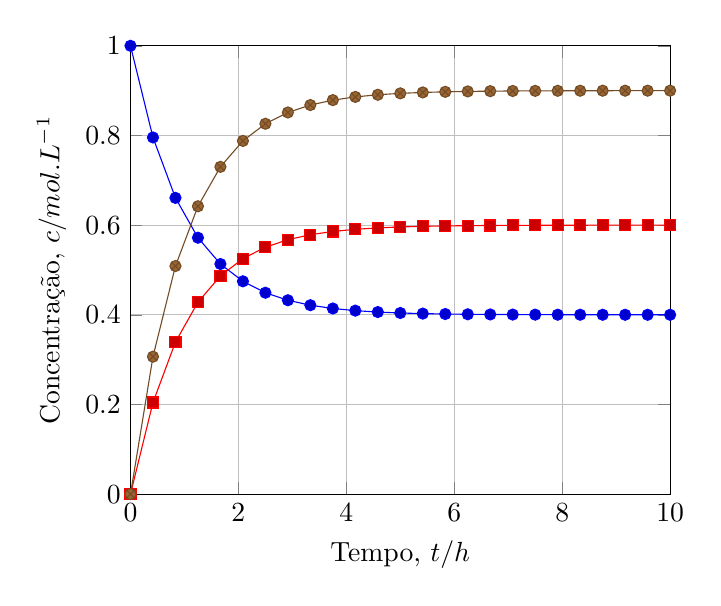
\begin{tikzpicture}
    \begin{axis}[
        xlabel={Tempo, $t/\unit{h}$},
        ylabel={Concentração, $c/\unit{mol.L^{-1}}$},
        grid=both,
        xmin=0, xmax=10,
        ymin=0, ymax=1,
        domain = 0:10,
    ]
    \addplot {
        0.4 + 0.6*exp(-x)
    };
    \addplot {
        0.6*(1 - exp(-x))
    };
    \addplot {
        0.9*(1 - exp(-x))
    };
    \end{axis}
\end{tikzpicture}

\caption{Figura do problema 2F39}
\end{figure}

\textbf{Determine} a constante de equilíbrio da reação balanceada com os menores coeficientes inteiros.

\end{problem}


\begin{problem}[
	id={2F40},
	path={/home/braun/Documents/Developer/braunchem/data/problems/Q2/2F/2F40}
]
As pressões parciais dos reagentes e produtos de uma reação foram monitoradas ao longo do tempo.

\begin{figure}
\centering
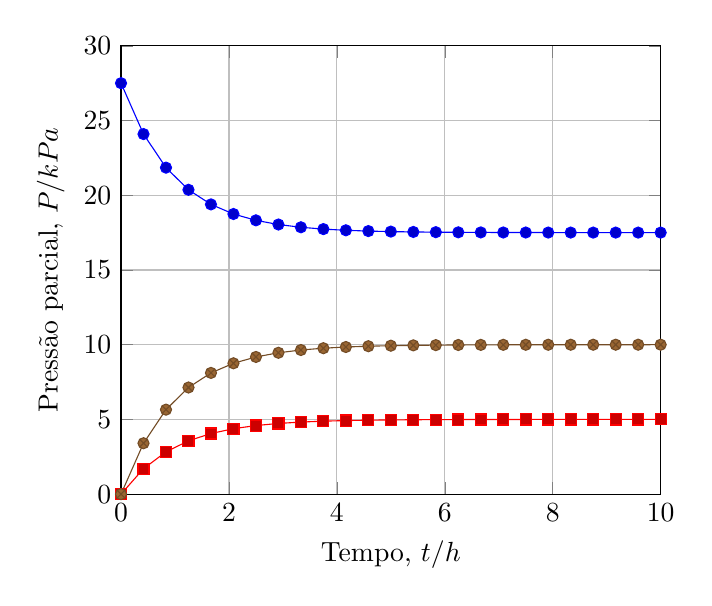
\begin{tikzpicture}
    \begin{axis}[
        xlabel={Tempo, $t/\unit{h}$},
        ylabel={Pressão parcial, $P/\unit{kPa}$},
        grid=both,
        ytick={0, 5, 10, 15, 20, 25, 30},
        xmin=0, xmax=10,
        ymin=0, ymax=30,
        domain = 0:10,
    ]
    \addplot {
        17.5 + 10*exp(-x)
    };
    \addplot {
        5*(1 - exp(-x))
    };
    \addplot {
        10*(1 - exp(-x))
    };
    \end{axis}
\end{tikzpicture}
\caption{Figura do problema 2F40.}
\end{figure}

\textbf{Determine} a constante de equilíbrio da reação balanceada com os menores coeficientes inteiros.

\end{problem}


\begin{problem}[
	id={2F41},
	path={/home/braun/Documents/Developer/braunchem/data/problems/Q2/2F/2F41}
]
Um reator é carregado com {\(\ce{PCl5}\)} e aquecido até {\(\qty{556}{\unit{K}}\)}, onde ocorre a reação: {\[
    \ce{ PCl5(g) <=> PCl3(g) + Cl2(g) } \quad K = 5
\]} No equilíbrio a pressão total é {\(\qty{15}{\unit{atm}}\)}.

\textbf{Determine} o grau de decomposição do {\(\ce{PCl5}\)} no equilíbrio.

\end{problem}


\begin{problem}[
	id={2F42},
	path={/home/braun/Documents/Developer/braunchem/data/problems/Q2/2F/2F42}
]
Um reator é carregado com {\(\ce{P4}\)} e aquecido até {\(\qty{1325}{\unit{K}}\)}, onde ocorre a reação: {\[
    \ce{ P4(g) <=> 2 P2(g) } \quad K = \num{0,1}
\]} No equilíbrio a pressão total é {\(\qty{1}{\unit{atm}}\)}.

\textbf{Determine} o grau de dissociação de {\(\ce{P4}\)} no equilíbrio.

\end{problem}


\begin{problem}[
	id={2F43},
	path={/home/braun/Documents/Developer/braunchem/data/problems/Q2/2F/2F43}
]
A {\(\qty{5000}{\unit{K}}\)} e {\(\qty{1}{\unit{atm}}\)}, {\(83\%\)} das moléculas de oxigênio em uma amostra estão dissociadas em oxigênio atômico.

\begin{enumerate}
\def\labelenumi{\alph{enumi}.}
\tightlist
\item
  \textbf{Determine} a constante de equilíbrio para a dissociação do oxigênio.
\item
  \textbf{Determine} a pressão em que {\(95\%\)} das moléculas de oxigênio estarão dissociadas em {\(\qty{5000}{\unit{K}}\)}.
\end{enumerate}

\end{problem}


\begin{problem}[
	id={2F44},
	path={/home/braun/Documents/Developer/braunchem/data/problems/Q2/2F/2F44}
]
Um reator é carregado com {\(\ce{CCl4}\)} e aquecido até {\(\qty{700}{\unit{\degree C}}\)}, onde ocorre a reação: {\[
    \ce{ CCl4(g) <=> C(s) + 2 Cl2(g) } \quad K = \num{0,8}
\]} No equilíbrio a pressão total é {\(\qty{1,2}{\unit{atm}}\)}.

\textbf{Determine} a pressão inicial de tetracloreto de carbono.

\end{problem}


\begin{problem}[
	id={2F45},
	path={/home/braun/Documents/Developer/braunchem/data/problems/Q2/2F/2F45}
]
Um balão de {\(\qty{1}{\unit{L}}\)} é carregado com {\(\qty{0,64}{\unit{bar}}\)} de fosfina. O sistema é mantido em {\(\qty{25}{\unit{\degree C}}\)} e
o equilíbrio é estabelecido: {\[
\ce{ 2 PH3(g) <=> 2 P(s) + 3 H2(g) }
\]} No equilíbrio a pressão total é {\(\qty{0,93}{\unit{atm}}\)}.

\begin{enumerate}
\def\labelenumi{\alph{enumi}.}
\tightlist
\item
  \textbf{Determine} a massa de fósforo produzida no equilíbrio.
\item
  \textbf{Determine} a constante de equilíbrio para essa reação.
\end{enumerate}

\end{problem}


\begin{problem}[
	id={2F46},
	path={/home/braun/Documents/Developer/braunchem/data/problems/Q2/2F/2F46}
]
Um cilindro é carregado com {\(\ce{N2O4}\)}. O sistema é mantido em {\(\qty{25}{\unit{\degree C}}\)} e o equilíbrio é estabelecido: {\[
\ce{ N2O4(g) <=> 2 NO2(g) }
\]} No equilíbrio, {\(\num{16}\%\)} do {\(\ce{N2O4}\)} está dissociado e a pressão total é {\(\qty{1,5}{\unit{atm}}\)}.

O volume do cilindro é aumentado até que a pressão total seja {\(\ce{1 atm}\)}.

\begin{enumerate}
\def\labelenumi{\alph{enumi}.}
\tightlist
\item
  \textbf{Determine} a constante de equilíbrio da reação.
\item
  \textbf{Determine} a pressão parcial de {\(\ce{NO2}\)} no equilíbrio.
\item
  \textbf{Determine} a fração de {\(\ce{N2O4}\)} dissociado no equilíbrio.
\end{enumerate}

\end{problem}


\begin{problem}[
	id={2F47},
	path={/home/braun/Documents/Developer/braunchem/data/problems/Q2/2F/2F47}
]
Um balão é carregado com {\(\qty{88}{\unit{g}}\)} de {\(\ce{SO3}\)}. O sistema é aquecido até {\(\qty{600}{\unit{\degree C}}\)} e o equilíbrio é
estabelecido: {\[
    \ce{ SO3(g) <=> SO2(g) + 1/2 O2(g) }
\]} No equilíbrio a densidade da fase gasosa é {\(\qty{1,6}{\unit{g.L^{-1}}}\)} e a pressão total é {\(\qty{1,8}{\unit{atm}}\)}.

\textbf{Determine} a constante de equilíbrio da reação.

\end{problem}


\begin{problem}[
	id={2F48},
	path={/home/braun/Documents/Developer/braunchem/data/problems/Q2/2F/2F48}
]
Um reator equipado com um pistão que se move livremente é carregado com {\(\ce{NOBr}\)}. A densidade da gás é {\(\qty{4,4}{\unit{g.L^{-1}}}\)}. O
sistema é mantido em {\(\qty{25}{\unit{\degree C}}\)} e o equilíbrio é estabelecido: {\[
    \ce{ 2 NOBr(g) <=> 2 NO(g) + Br2(g) }
\]} No equilíbrio a densidade da fase gasosa é {\(\qty{4,0}{\unit{g.L^{-1}}}\)}.

\begin{enumerate}
\def\labelenumi{\alph{enumi}.}
\tightlist
\item
  \textbf{Determine} a constante de equilíbrio dessa reação.
\item
  \textbf{Explique} o efeito da adição de argônio ao reator.
\end{enumerate}

\end{problem}


\begin{problem}[
	id={2F49},
	path={/home/braun/Documents/Developer/braunchem/data/problems/Q2/2F/2F49}
]
Um reservatório de {\(\qty{6}{\unit{L}}\)} é carregado com {\(\qty{79,2}{\unit{g}}\)} de gelo seco e {\(\qty{30}{\unit{g}}\)} de carvão mineral em pó.
O sistema é aquecido até {\(\qty{1000}{\unit{K}}\)} e o equilíbrio é estabelecido: {\[
    \ce{ CO2(g) + C(s) <=> 2 CO(g) }
\]} No equilíbrio a densidade da fase gasosa é {\(\qty{14}{\unit{g.L^{-1}}}\)}. Em {\(\qty{1100}{\unit{K}}\)}, a constante de equilíbrio da reação é
{\(22\)}.

\begin{enumerate}
\def\labelenumi{\alph{enumi}.}
\tightlist
\item
  \textbf{Determine} a constante de equilíbrio da reação a {\(\qty{1000}{\unit{K}}\)}
\item
  \textbf{Classifique} a reação como endotérmica ou exotérmica.
\end{enumerate}

\end{problem}


\begin{problem}[
	id={2F50},
	path={/home/braun/Documents/Developer/braunchem/data/problems/Q2/2F/2F50}
]
Em fase gasosa, o ácido acético sofre dimerização conforme a reação: {\[
    \ce{ 2 CH3COOH(g) <=> (CH3COOH)2(g) }
\]} Em um recipiente de {\(\qty{20}{\unit{mL}}\)} em {\(\qty{160}{\unit{\degree C}}\)} foram coleados {\(\qty{40,7}{\unit{mg}}\)} de vapor de ácido
acético sob {\(\qty{1}{\unit{atm}}\)}. Quando o mesmo experimento foi realizado em {\(\qty{200}{\unit{\degree C}}\)}, {\(\qty{33,4}{\unit{mg}}\)} de
gás foram coletados no mesmo recipiente de {\(\qty{20}{\unit{mL}}\)}.

\begin{enumerate}
\def\labelenumi{\alph{enumi}.}
\tightlist
\item
  \textbf{Determine} a constante de equilíbrio para a dimerização do ácido acético em {\(\qty{160}{\unit{\degree C}}\)}.
\item
  \textbf{Determine} a constante de equilíbrio para a dimerização do ácido acético em {\(\qty{200}{\unit{\degree C}}\)}.
\item
  \textbf{Determine} a entalpia de dimerização do ácido acético.
\end{enumerate}

\end{problem}


\begin{problem}[
	id={2F51},
	path={/home/braun/Documents/Developer/braunchem/data/problems/Q2/2F/2F51}
]
Um balão de {\(\qty{1}{\unit{L}}\)} foi carregado com {\(\qty{4,8}{\unit{g}}\)} de metanol. O sistema é aquecido até {\(\qty{250}{\unit{\degree C}}\)}
e o equilíbrio é estabelecido: {\[
    \ce{ CH3OH(g) <=> CO(g) + 2 H2(g) }
\]} Um frasco é preenchido por um pequeno orifício na lateral do balão. A quantidade de hidrogênio que efunde para o frasco é {\(\num{32}\)} vezes
maior que a quantidade de metanol.

\begin{enumerate}
\def\labelenumi{\alph{enumi}.}
\tightlist
\item
  \textbf{Determine} a razão entre a quantidade de hidrogênio e metanol na mistura em equilíbrio.
\item
  \textbf{Determine} a constante de equilíbrio para essa reação.
\end{enumerate}

\end{problem}


\begin{problem}[
	id={2F52},
	path={/home/braun/Documents/Developer/braunchem/data/problems/Q2/2F/2F52}
]
Um balão de {\(\qty{250}{\unit{mL}}\)} foi carregado com {\(\qty{420}{\unit{Torr}}\)} de uma mistura equimolar de monóxido de carbono e vapor d'água.
O sistema é aquecido até {\(\qty{700}{\unit{\degree C}}\)} e o equilíbrio é estabelecido: {\[
    \ce{ CO(g) + H2O(g) <=> CO2(g) + 2 H2(g) }
\]} Um frasco é preenchido por um pequeno orifício na lateral do balão. A quantidade de hidrogênio que efunde para o frasco é {\(\num{2,25}\)} vezes
maior que a quantidade de vapor d'água.

\begin{enumerate}
\def\labelenumi{\alph{enumi}.}
\tightlist
\item
  \textbf{Determine} a razão entre a quantidade de hidrogênio e vapor d'água na mistura em equilíbrio.
\item
  \textbf{Determine} a constante de equilíbrio para essa reação.
\end{enumerate}

\end{problem}


\begin{problem}[
	id={2F53},
	path={/home/braun/Documents/Developer/braunchem/data/problems/Q2/2F/2F53}
]
Em solução de tetracloreto de carbono, o tetracloreto de vanádio sofre dimerização formando {\(\ce{V2Cl8}\)}: {\[
    \ce{ 2 VCl4(org) <=> V2Cl8(org) }
\]} Em um experimento, {\(\qty{6,76}{\unit{g}}\)} de {\(\ce{VCl4}\)} foram dissolvidos em {\(\qty{100}{\unit{g}}\)} de tetracloreto de carbono em
{\(\qty{0}{\unit{\degree C}}\)}. Após certo tempo, a mistura alcançou o equilíbrio, sendo a densidade {\(\qty{1,78}{\unit{g.cm^{-3}}}\)}. O ponto de
fusão da solução é {\(\qty{-29}{\unit{\degree C}}\)}

\begin{enumerate}
\def\labelenumi{\alph{enumi}.}
\tightlist
\item
  \textbf{Determine} o grau de dimerização do tetracloreto de vanádio.
\item
  \textbf{Determine} a constante de equilíbrio de dimerização.
\end{enumerate}
\paragraph{Dados}\small 
\begin{datalist}
[start = 1](2)\item $k_\mathrm{c}(\ce{CCl4}) = \qty{30}{\tfrac{\unit{K.kg}}{\unit{mol}}}$
\item $T_\mathrm{fus}(\ce{CCl4}) = \qty{-23}{\unit{\degree C}}$
\end{datalist}

\end{problem}


\begin{problem}[
	id={2F54},
	path={/home/braun/Documents/Developer/braunchem/data/problems/Q2/2F/2F54}
]
O propionato de metila, {\(\ce{CH3CH2COOCH3}\)}, sofre hidrólise em solução aquosa formando ácido propanoico e metanol, conforme a reação: {\[
    \ce{ RCOOCH3(aq) + H2O(l) <=> RCOOH(aq) + CH3OH(aq) }
\]} Em um experimento, {\(\qty{880}{\unit{mg}}\)} de propionato de metila foram dissolvidos em {\(\qty{100}{\unit{mL}}\)} de água em
{\(\qty{25}{\unit{\degree C}}\)}. Após certo tempo, a mistura alcançou o equilíbrio. O ponto de fusão da solução é
{\(\qty{-0,23}{\unit{\degree C}}\)}. Desconsidere a ionização do ácido carboxílico formado.

\begin{enumerate}
\def\labelenumi{\alph{enumi}.}
\tightlist
\item
  \textbf{Determine} o grau de hidrólise do éster.
\item
  \textbf{Determine} a constante de equilíbrio de hidrólise do éster.
\end{enumerate}
\paragraph{Dados}\small 
\begin{datalist}
[start = 1](2)\item $k_\mathrm{c}(\ce{H2O}) = \qty{1.9}{\tfrac{\unit{K.kg}}{\unit{mol}}}$
\end{datalist}

\end{problem}


\begin{problem}[
	id={2F55},
	path={/home/braun/Documents/Developer/braunchem/data/problems/Q2/2F/2F55}
]
Em um reator mantido em temperatura constante ocorre a reação: {\[
    \ce{ N2O4(g) <=> 2 NO2(g) }
\]} No equilíbrio, a pressão parcial de {\(\ce{N2O4}\)} era {\(\qty{0,34}{\unit{atm}}\)} e a de {\(\ce{NO2}\)} era {\(\qty{2}{\unit{atm}}\)}. O volume
do recipiente é duplicado mantendo a temperatura constante e o equilíbrio é reestabelecido.

\begin{enumerate}
\def\labelenumi{\alph{enumi}.}
\tightlist
\item
  \textbf{Determine} a constante de equilíbrio da reação.
\item
  \textbf{Determine} a pressão parcial de {\(\ce{N2O4}\)} no equilíbrio.
\end{enumerate}

\end{problem}


\begin{problem}[
	id={2F56},
	path={/home/braun/Documents/Developer/braunchem/data/problems/Q2/2F/2F56}
]
Sob {\(\qty{1}{\unit{atm}}\)}, {\(\num{0,5}\%\)} do pentóxido de nitrogênio em um cilindro está decomposto devido a reação: {\[
    \ce{ 2 N2O5(g) <=> 4 NO2(g) + O2(g) }
\]} O volume do cilindro é aumentado em dez vezes e o equilíbrio é reestabelecido.

\begin{enumerate}
\def\labelenumi{\alph{enumi}.}
\tightlist
\item
  \textbf{Determine} a pressão parcial de {\(\ce{O2}\)} no equilíbrio.
\item
  \textbf{Determine} a fração de {\(\ce{N2O5}\)} que sofre decomposição devido ao aumento do volume.
\end{enumerate}

\end{problem}


\begin{problem}[
	id={2F57},
	path={/home/braun/Documents/Developer/braunchem/data/problems/Q2/2F/2F57}
]
Um reator de {\(\qty{5}{\unit{L}}\)} é carregado com {\(\qty{2}{\unit{mol}}\)} de {\(\ce{NH3}\)}, {\(\qty{2}{\unit{mol}}\)} de {\(\ce{H2S}\)} e
{\(\qty{2}{\unit{mol}}\)} de {\(\ce{NH4HS}\)}. O sistema é mantido em {\(\qty{35}{\unit{\degree C}}\)} e o equilíbrio é estabelecido: {\[
    \ce{ NH3(g) + H2S(g) <=> NH4HS(s) } \quad K_\mathrm{c} = 400
\]}

\begin{enumerate}
\def\labelenumi{\alph{enumi}.}
\tightlist
\item
  \textbf{Determine} pressão parcial de {\(\ce{H2S}\)} no equilíbrio.
\item
  \textbf{Determine} a massa de {\(\ce{NH4HS}\)} no equilíbrio.
\end{enumerate}

\end{problem}


\begin{problem}[
	id={2F58},
	path={/home/braun/Documents/Developer/braunchem/data/problems/Q2/2F/2F58}
]
Uma amostra de {\(\qty{25}{\unit{g}}\)} de carbamato de amônio, {\(\ce{NH4(NH2CO2)}\)}, é adicionada em um recipiente de {\(\qty{250}{\unit{mL}}\)}. O
sistema é mantido em {\(\qty{25}{\unit{\degree C}}\)} e o equilíbrio é estabelecido: {\[
\ce{ NH4(NH2CO2)(s) <=> 2 NH3(g) + CO2(g) }
\]} No equilíbrio, a massa de dióxido de carbono é {\(\qty{17,4}{\unit{mg}}\)}.

\textbf{Determine} a constante de equilíbrio {\(K_\mathrm{c}\)} da reação.

\end{problem}


\begin{problem}[
	id={2F59},
	path={/home/braun/Documents/Developer/braunchem/data/problems/Q2/2F/2F59}
]
Um reator de {\(\qty{1}{\unit{L}}\)} é carregado com {\(\qty{10}{\unit{g}}\)} de bicarbonato de sódio. O sistema é aquecido até
{\(\qty{125}{\unit{\degree C}}\)} e o equilíbrio é estabelecido: {\[
    \ce{ 2 NaHCO3(s) <=> Na2CO3(s) + CO2(g) + H2O(g) }
\]}

\begin{enumerate}
\def\labelenumi{\alph{enumi}.}
\tightlist
\item
  \textbf{Determine} a pressão parcial de {\(\ce{CO2}\)} no equilíbrio.
\item
  \textbf{Determine} a massa de bicarbonato de sódio no equilíbrio.
\item
  \textbf{Determine} o volume mínimo do reator necessário para a decomposição de todo o bicarbonato.
\end{enumerate}

\end{problem}


\begin{problem}[
	id={2F60},
	path={/home/braun/Documents/Developer/braunchem/data/problems/Q2/2F/2F60}
]
Quando {\(\ce{NaHCO3}\)} sólido é colocado em um recipiente rígido de {\(\qty{2,5}{\unit{L}}\)} e aquecido até {\(\qty{160}{\unit{\degree C}}\)} o
equilíbrio é estabelecido: {\[
    \ce{ 2 NaHCO3(s) <=> Na2CO3(s) + CO2(g) + H2O(g) }
\]} No equilíbrio, a pressão total é {\(\qty{8}{\unit{bar}}\)}.

Em um segundo experimento, é adicionada a mesma massa de sólido em um recipiente de mesmo volume com {\(\qty{1}{\unit{bar}}\)} de {\(\ce{CO2}\)}.

\begin{enumerate}
\def\labelenumi{\alph{enumi}.}
\tightlist
\item
  \textbf{Determine} a constante de equilíbrio da reação.
\item
  \textbf{Determine} a pressão parcial de {\(\ce{CO2}\)} no equilíbrio no segundo experimento.
\end{enumerate}

\end{problem}


\begin{problem}[
	id={2F61},
	path={/home/braun/Documents/Developer/braunchem/data/problems/Q2/2F/2F61}
]
Uma alíquota de {\(\qty{25}{\unit{mL}}\)} de uma solução aquosa contendo {\(\qty{2}{\unit{mg}}\)} de iodo é agitada com {\(\qty{5}{\unit{mL}}\)} de
{\(\ce{CCl4}\)} e, em seguida, as soluções se separam. O equilíbrio de partição do iodo entre água e {\(\ce{CCl4}\)} é: {\[
    \ce{ I2(aq) <=> I2(org) } \quad D = \num{82}
\]}

\begin{enumerate}
\def\labelenumi{\alph{enumi}.}
\tightlist
\item
  \textbf{Determine} a quantidade de iodo remanescente na solução aquosa após a extração.
\item
  \textbf{Determine} o número de etapas de extração para que a concentração de iodo na fase aquosa seja inferior a {\(\qty{1}{\unit{ppm}}\)}.
\end{enumerate}

\end{problem}


\begin{problem}[
	id={2F62},
	path={/home/braun/Documents/Developer/braunchem/data/problems/Q2/2F/2F62}
]
A penicilina pode ser purificada por extração. O equilibrio de partição da penicilina-F entre éter isopropílico e uma solução aquosa de fosfato é: {\[
    \ce{ \text{penicilina-F}(aq) <=> \text{penicilina-F}(org) }
\quad D_\mathrm{F} = \num{0,35}
\]} O equilíbrio de partição correspondente para a penicilina-G é: {\[
    \ce{ \text{penicilina-G}(aq) <=> \text{penicilina-G}(org) }
\quad D_\mathrm{G} = \num{0,70}
\]} Uma amostra de penicilina-G possui {\(\num{10}\%\)} de penicilina-F como impureza. Essa amostra é dissolvida na solução aquosa de fosfato e
extraída com o mesmo volume de éter isopropílico. O processo de extração é repetido até que a fração de impureza na penicilina seja inferior a
{\(\num{4}\%\)}.

\begin{enumerate}
\def\labelenumi{\alph{enumi}.}
\tightlist
\item
  \textbf{Determine} a fração de impureza após a primeira extração.
\item
  \textbf{Determine} o número de etapas de extração realizadas.
\item
  \textbf{Determine} a fração da penicilina-G inicial remanescente na solução aquosa após as extrações.
\end{enumerate}

\end{problem}


\begin{problem}[
	id={2F63},
	path={/home/braun/Documents/Developer/braunchem/data/problems/Q2/2F/2F63}
]
A constante de equilíbrio para uma reação é {\(\num{8,84}\)} em {\(\qty{25}{\unit{\degree C}}\)} e {\(\num{0,0325}\)} em
{\(\qty{75}{\unit{\degree C}}\)}.

\begin{enumerate}
\def\labelenumi{\alph{enumi}.}
\tightlist
\item
  \textbf{Determine} a temperatura em que a constante de equilíbrio da reação é {\(K = 1\)}.
\item
  \textbf{Determine} a entropia padrão de reação.
\end{enumerate}

\end{problem}


\begin{problem}[
	id={2F64},
	path={/home/braun/Documents/Developer/braunchem/data/problems/Q2/2F/2F64}
]
Um reator contém uma mistura dos gases metilpropeno, \emph{cis}-but-2-eno e \emph{trans}-but-2-eno em equilíbrio.

\textbf{Determine} a fração de cada composto no equilíbrio.
\paragraph{Dados}\small 
\begin{datalist}
[start = 1](2)\item $\Delta G_\text{f}^\circ(\text{\textit{cis}-buteno}) = \qty{66}{\tfrac{\unit{kJ}}{\unit{mol}}}$
\item $\Delta G_\text{f}^\circ(\text{\textit{trans}-buteno}) = \qty{63}{\tfrac{\unit{kJ}}{\unit{mol}}}$
\item $\Delta G_\text{f}^\circ(\text{metilpropeno}) = \qty{58}{\tfrac{\unit{kJ}}{\unit{mol}}}$
\end{datalist}

\end{problem}


\begin{problem}[
	id={2F65},
	path={/home/braun/Documents/Developer/braunchem/data/problems/Q2/2F/2F65}
]
Quando o carbonato de prata hidratado é seco com uma corrente de ar quente, o ar deve ter uma concentração mínima de {\(\ce{CO2}\)} para evitar a
decomposição deste, conforme a reação: {\[
    \ce{ Ag2CO3(s) -> Ag2O(s) + CO2(g) } \quad \Delta
H^\circ_\mathrm{r} = \qty{+80}{\tfrac{\unit{kJ}}{\unit{mol}}}
\]} Em {\(\qty{25}{\unit{\degree C}}\)}, a pressão parcial mínima de {\(\ce{CO2}\)} para que não ocorra decomposição é
{\(\qty{6,2e-3}{\unit{Torr}}\)}.

\textbf{Determine} a pressão parcial mínima de {\(\ce{CO2}\)} para que não ocorra decomposição em {\(\qty{110}{\unit{\degree C}}\)}.

\end{problem}


\begin{problem}[
	id={2F66},
	path={/home/braun/Documents/Developer/braunchem/data/problems/Q2/2F/2F66}
]
Quando o carbonato de cálcio é aquecido ocorre a reação: {\[
    \ce{ CaCO3(s) <=> CaO(s) + CO2(g) }
\]} A constante de equilíbrio dessa reação pode ser calculada entre {\(\qty{850}{\unit{\degree C}}\)} e {\(\qty{950}{\unit{\degree C}}\)} pela
relação: {\[
    \ln K = \num{7,3} - \dfrac{ \num{8500} }{ T/\unit{K} }
\]}

\begin{enumerate}
\def\labelenumi{\alph{enumi}.}
\tightlist
\item
  \textbf{Determine} a temperatura necessária para a decomposição de todo o carbonato de cálcio em uma amostra sob {\(\qty{1}{\unit{atm}}\)}.
\item
  \textbf{Determine} a entalpia padrão de reação.
\item
  \textbf{Determine} a entropia padrão de reação.
\end{enumerate}

\end{problem}


\begin{problem}[
	id={2F67},
	path={/home/braun/Documents/Developer/braunchem/data/problems/Q2/2F/2F67}
]
Um reator de {\(\qty{10}{\unit{L}}\)} é carregado com {\(\qty{1}{\unit{atm}}\)} de gás fosgênio, {\(\ce{COCl2}\)}. O sistema é aquecido até
{\(\qty{1000}{\unit{K}}\)} e os equilíbrios são estabelecidos: {\[
\begin{aligned}
    \ce{ COCl2(g) &<=> CO(g) + Cl2(g) } && K_1 =
\num{8,0e-2} \\
    \ce{ Cl2(g) &<=> 2 Cl(g) } && K_2 = \num{2,5e-5}
\end{aligned}
\]}

\begin{enumerate}
\def\labelenumi{\alph{enumi}.}
\tightlist
\item
  \textbf{Determine} a pressão parcial de {\(\ce{Cl2}\)} no reservatório.
\item
  \textbf{Determine} a pressão parcial de {\(\ce{Cl}\)} no reservatório.
\end{enumerate}

\end{problem}


\begin{problem}[
	id={2F68},
	path={/home/braun/Documents/Developer/braunchem/data/problems/Q2/2F/2F68}
]
Bromo líquido é adicionado a um reservatório. O sistema é mantido em {\(\qty{25}{\unit{\degree C}}\)} e os equilíbrios são estabelecidos: {\[
\begin{aligned}
    \ce{ Br2(l) &<=> Br2(g) } \\
    \ce{ Br2(g) &<=> 2 Br(g) }
\end{aligned}
\]} Deseja-se coletar {\(\qty{0,01}{\unit{mol}}\)} de bromo gasoso enchendo um frasco sob vácuo com o vapor de bromo do reservatório.

\begin{enumerate}
\def\labelenumi{\alph{enumi}.}
\tightlist
\item
  \textbf{Determine} a pressão parcial do bromo atômico no equilíbrio.
\item
  \textbf{Determine} o volume do frasco necessário para coletar a quantidade de bromo desejada.
\end{enumerate}
\paragraph{Dados}\small 
\begin{datalist}
[start = 1](2)\item $\Delta G_\mathrm{f}^{\circ}(\ce{Br2,\,\text{g}}) = \qty{3.11}{\tfrac{\unit{kJ}}{\unit{mol}}}$
\item $\Delta G_\mathrm{f}^{\circ}(\ce{Br,\,\text{g}}) = \qty{82.4}{\tfrac{\unit{kJ}}{\unit{mol}}}$
\end{datalist}

\end{problem}

\section*{Desafios}

\begin{problem}[
	id={2F69},
	path={/home/braun/Documents/Developer/braunchem/data/problems/Q2/2F/2F69}
]
Um reator de {\(\qty{1}{\unit{L}}\)} é carregado com {\(\qty{60}{\unit{g}}\)} de {\(\ce{NO}\)} e {\(\ce{71 g}\)} de {\(\ce{Cl2}\)}. O sistema é
aquecido até {\(\qty{35}{\unit{\degree C}}\)} e o equilíbrio é estabelecido: {\[
    \ce{ 2 NOCl(g) <=> 2 NO(g) + Cl2(g) } \quad K_\mathrm{c} =
\num{1,6e-5}
\]}

\begin{enumerate}
\def\labelenumi{\alph{enumi}.}
\tightlist
\item
  \textbf{Determine} a concentração de {\(\ce{NOCl}\)} no equilíbrio.
\item
  \textbf{Determine} a concentração de {\(\ce{NO}\)} no equilíbrio.
\end{enumerate}

\end{problem}


\begin{problem}[
	id={2F70},
	path={/home/braun/Documents/Developer/braunchem/data/problems/Q2/2F/2F70}
]
Um balão é carregado com {\(\qty{100}{\unit{Torr}}\)} de {\(\ce{NO}\)} e {\(\qty{40}{\unit{Torr}}\)} de {\(\ce{Br2}\)}. O sistema é mantido em
{\(\qty{300}{\unit{K}}\)} e o equilíbrio é estabelecido: {\[
\ce{ 2 NO(g) + Br2(g) <=> 2 NOBr(g) }
\]} No equilíbrio a pressão total é {\(\qty{110}{\unit{Torr}}\)}.

Em outro experimento, {\(\qty{0,6}{\unit{atm}}\)} de uma mistura equimolar de {\(\ce{NO}\)} e {\(\ce{Br2}\)} são carregados em um balão em
{\(\qty{300}{\unit{K}}\)}.

\begin{enumerate}
\def\labelenumi{\alph{enumi}.}
\tightlist
\item
  \textbf{Determine} a constante de equilíbrio da reação.
\item
  \textbf{Determine} a pressão parcial de {\(\ce{NOBr}\)} em equilíbrio no segundo experimento.
\end{enumerate}

\end{problem}


\begin{problem}[
	id={2F71},
	path={/home/braun/Documents/Developer/braunchem/data/problems/Q2/2F/2F71}
]
Um reator de {\(\qty{22,4}{\unit{L}}\)} é carregado com {\(\qty{100}{\unit{g}}\)} de carbonato de cálcio e {\(\qty{12}{\unit{g}}\)} de carbono. O
sistema é aquecido até {\(\qty{820}{\unit{\degree C}}\)} e os equilíbrios são estabelecidos: {\[
\begin{aligned}
    \ce{ CaCO3(s) &<=> CaO(s) + CO2(g) } && K_1 =
\num{0,2} \\
    \ce{ CO2(g) + C(s) &<=> 2 CO(g) } && K_2 =
\num{2,0}
\end{aligned}
\]}

\begin{enumerate}
\def\labelenumi{\alph{enumi}.}
\tightlist
\item
  \textbf{Determine} a quantidade de {\(\ce{CO2}\)} no equilíbrio.
\item
  \textbf{Determine} a quantidade de {\(\ce{C}\)} no equilíbrio.
\item
  \textbf{Determine} o volume mínimo do reator necessário para a decomposição de todo o carbonato.
\end{enumerate}

\end{problem}


\begin{problem}[
	id={2F72},
	path={/home/braun/Documents/Developer/braunchem/data/problems/Q2/2F/2F72}
]
Um reator é carregado com sulfato de ferro(II), {\(\ce{FeSO4}\)}. O sistema é aquecido até {\(\qty{920}{\unit{K}}\)} e os equilíbrios são
estabelecidos: {\[
\begin{aligned}
    \ce{ 2 FeSO4(g) &<=> Fe2O3(s) + SO3(g) + SO2(g) }
&& K_1 \\
    \ce{ 2 SO3(g) &<=> 2 SO2(g) + O2(g) } && K_2
\end{aligned}
\]} No equilíbrio, a pressão parcial de oxigênio é {\(\qty{0,0275}{\unit{atm}}\)} e a pressão total é {\(\qty{0,836}{\unit{atm}}\)}.

\begin{enumerate}
\def\labelenumi{\alph{enumi}.}
\tightlist
\item
  \textbf{Determine} a constante de equilíbrio {\(K_1\)}
\item
  \textbf{Determine} a constante de equilíbrio {\(K_2\)}
\end{enumerate}

\end{problem}


\begin{problem}[
	id={2F73},
	path={/home/braun/Documents/Developer/braunchem/data/problems/Q2/2F/2F73}
]
Um reator de {\(\qty{10}{\unit{L}}\)} é carregado com {\(\qty{24}{\unit{g}}\)} de carbono e {\(\qty{108}{\unit{g}}\)} de água. O sistema é aquecido
até {\(\qty{215}{\unit{\degree C}}\)} e os equilíbrios são estabelecidos: {\[
\begin{aligned}
    \ce{ C(s) + H2O(g) &<=> CO(g) + H2(g) } && K_1 =
\num{0,4} \\
    \ce{ CO(g) + H2O(g) &<=> CO2(g) + H2(g) } && K_2
\end{aligned}
\]} No equilíbrio, a pressão total é {\(\qty{28,8}{\unit{atm}}\)}.

\begin{enumerate}
\def\labelenumi{\alph{enumi}.}
\tightlist
\item
  \textbf{Determine} a quantidade de vapor d'água no equilíbrio.
\item
  \textbf{Determine} a constante de equilíbrio {\(K_2\)}.
\item
  \textbf{Determine} o volume mínimo do reator necessário para a decomposição de todo o carbono.
\end{enumerate}

\end{problem}


\begin{problem}[
	id={2F74},
	path={/home/braun/Documents/Developer/braunchem/data/problems/Q2/2F/2F74}
]
Um ácido dicarboxílico, {\(\ce{A}\)}, é misturado com etanol. O sistema é mantido em {\(\qty{25}{\unit{\degree C}}\)} e os equilíbrios são
estabelecidos: {\[
\begin{aligned}
    \ce{ A(l) + EtOH(l) &<=> M(l) + H2O(l) } && K_1 =
20 \\
    \ce{ M(l) + EtOH(l) &<=> D(l) + H2O(l) } && K_2 =
20
\end{aligned}
\]}

\begin{enumerate}
\def\labelenumi{\alph{enumi}.}
\tightlist
\item
  \textbf{Determine} o rendimento máximo para a conversão do ácido dicarboxílico no monoéster, {\(\ce{M}\)}.
\item
  \textbf{Determine} a razão entre as frações molares de etanol e do ácido dicarboxílico na mistura inicial para que a fração molar de monoéster no
  equilíbrio seja máxima.
\end{enumerate}

\end{problem}

\section*{Gabarito}

\subsection*{Problemas}
\small 
\begin{mcanswers}
[start = 1](6)\answer \choicebox{B}
\answer \choicebox{C}
\answer \choicebox{D}
\answer \choicebox{D}
\answer \choicebox{B}
\answer \choicebox{B}
\answer \choicebox{B}
\answer \choicebox{C}
\answer \choicebox{B}
\answer \choicebox{E}
\answer \choicebox{C}
\answer \choicebox{C}
\answer \choicebox{E}
\answer \choicebox{A}
\answer \choicebox{A}
\answer \choicebox{E}
\answer \choicebox{A}
\answer \choicebox{D}
\answer \choicebox{C}
\answer \choicebox{A}
\answer \choicebox{E}
\answer \choicebox{A}
\answer \choicebox{A}
\answer \choicebox{C}
\answer \choicebox{C}
\answer \choicebox{C}
\answer \choicebox{D}
\answer \choicebox{C}
\answer \choicebox{D}
\answer \choicebox{B}
\answer \choicebox{D}
\answer \choicebox{D}
\answer \choicebox{D}
\answer \choicebox{C}
\answer \choicebox{C}
\answer \choicebox{D}
\answer \choicebox{C}
\answer \choicebox{A}
\end{mcanswers}

\subsection*{Problemas cumulativos}
\small 
\begin{answers}
[start = 39]\item \(\num{1,64}\)

\item \(\num{0,016}\)

\item \(50\%\)

\item \(16\%\)

\item 
\begin{answers}
[start = 1]\item \(\num{8,9}\)

\item \(\qty{0,24}{\unit{atm}}\)

\end{answers}

\item \(\qty{0,9}{\unit{atm}}\)

\item 
\begin{answers}
[start = 1]\item \(\qty{720}{\unit{mg}}\)

\item \(\num{183}\)

\end{answers}

\item 
\begin{answers}
[start = 1]\item \(\num{0,16}\)

\item \(\qty{0,33}{\unit{atm}}\)

\item \(\num{20}\%\)

\end{answers}

\item \(\num{0,86}\)

\item 
\begin{answers}
[start = 1]\item \(\num{2,33e-4}\)

\item O equilíbrio é deslocado, formando mais produtos.

\end{answers}

\item 
\begin{answers}
[start = 1]\item \(\num{6,76}\)

\item Endotérmica.

\end{answers}

\item 
\begin{answers}
[start = 1]\item \(\num{0,324}\)

\item \(\num{0,095}\)

\item \(\qty{-52}{\unit{kJ.mol^{-1}}}\)

\end{answers}

\item 
\begin{answers}
[start = 1]\item \(\num{8}\)

\item \(\num{0,23}\)

\end{answers}

\item 
\begin{answers}
[start = 1]\item \(\num{0,75}\)

\item \(\num{0,5625}\)

\end{answers}

\item 
\begin{answers}
[start = 1]\item \(85\%\)

\item \(\num{33}\)

\end{answers}

\item 
\begin{answers}
[start = 1]\item \(20\%\)

\item \(\num{0,005}\)

\end{answers}

\item 
\begin{answers}
[start = 1]\item \(\num{4,2}\)

\item \(\qty{0,12}{\unit{atm}}\)

\end{answers}

\item 
\begin{answers}
[start = 1]\item \(\qty{4e-3}{\unit{atm}}\)

\item \(2\%\)

\end{answers}

\item 
\begin{answers}
[start = 1]\item \(\qty{1,3}{\unit{atm}}\)

\item \(\qty{192}{\unit{g}}\)

\end{answers}

\item \(\num{2,3e-4}\)

\item 
\begin{answers}
[start = 1]\item \(\qty{0,5}{\unit{atm}}\)

\item \(\qty{7,5}{\unit{g}}\)

\item \(\qty{3,9}{\unit{L}}\)

\end{answers}

\item 
\begin{answers}
[start = 1]\item \(\num{16}\)

\item \(\qty{4,5}{\unit{bar}}\)

\end{answers}

\item 
\begin{answers}
[start = 1]\item \(\qty{0,11}{\unit{mg}}\)

\item 4 etapas

\end{answers}

\item 
\begin{answers}
[start = 1]\item \(\num{8,1}\%\)

\item 5 etapas

\item \(\num{23}\%\)

\end{answers}

\item 
\begin{answers}
[start = 1]\item \(\qty{310}{\unit{K}}\)

\item \(\qty{310}{\unit{J.mol^{-1}.K^{-1}}}\)

\end{answers}

\item \(87\%\) metilpropeno, \(3\%\) \emph{cis}-but-2-eno e \(10\%\) \emph{trans}-but-2-eno.

\item \(\qty{7,5}{\unit{Torr}}\)

\item 
\begin{answers}
[start = 1]\item \(\qty{1160}{\unit{K}}\)

\item \(\qty{61}{\unit{J.K^{-1}.mol^{-1}}}\)

\item \(\qty{70}{\unit{kJ.mol^{-1}}}\)

\end{answers}

\item 
\begin{answers}
[start = 1]\item \(\qty{0,25}{\unit{atm}}\)

\item \(\qty{0,0025}{\unit{atm}}\)

\end{answers}

\item 
\begin{answers}
[start = 1]\item \(\qty{3,6e-15}{\unit{atm}}\)

\item \(\qty{846}{\unit{mL}}\)

\end{answers}

\end{answers}

\subsection*{Desafios}
\small 
\begin{answers}
[start = 69]\item 
\begin{answers}
[start = 1]\item \(\qty{1,95}{\unit{mol.L^{-1}}}\)

\item \(\qty{0,05}{\unit{mol.L^{-1}}}\)

\end{answers}

\item 
\begin{answers}
[start = 1]\item \(\num{171}\)

\item \(\qty{0,22}{\unit{atm}}\)

\end{answers}

\item 
\begin{answers}
[start = 1]\item \(\qty{0,05}{\unit{mol}}\)

\item \(\qty{0,91}{\unit{mol}}\)

\item \(\qty{192}{\unit{L}}\)

\end{answers}

\item 
\begin{answers}
[start = 1]\item \(\num{0,16}\)

\item \(\num{0,048}\)

\end{answers}

\item 
\begin{answers}
[start = 1]\item \(\qty{3,7}{\unit{mol}}\)

\item \(4\)

\item \(\qty{70}{\unit{L}}\)

\end{answers}

\item 
\begin{answers}
[start = 1]\item \(\dfrac{1}{1 + 2\sqrt{\dfrac{K_2}{K_1}}} = \dfrac{1}{3}\)

\item \(1 + \dfrac{1}{\sqrt{K_1K_2}} = \num{1,05}\)

\end{answers}

\end{answers}
